\NeedsTeXFormat{LaTeX2e}
\documentclass[10pt,a4paper]{book}

\usepackage{test}
\usepackage{etoolbox}
\usepackage{tikz}
\usepackage{xcolor,colortbl}
\selectlanguage{russian}
\graphicspath{{pic}}

%--- Здесь можно добавить свои команды --------
%\def\Algo500{\mbox{Algo500}}
%\def\AlgoWiki{\mbox{AlgoWiki}}
%\def\CompZoo{\mbox{CompZoo}}
%\def\CompBase{\mbox{CompBase}}
%\def\PerfData{\mbox{PerfData}}
%\def\RatingLists{\mbox{RatingLists}}


\begin{document}
    %===========================  ШАПКА СТАТЬИ =================================
    \Article{\vspace*{8mm}\par Параметрическое исследование оригинальной конструкции клапана Теслы}
    {\newpage eng text}
    
    \Abstract{В данной работе рассматривалась оригинальная конструкция гидродинамического диода в котором основным исследуемым параметром был выбран угол наклона отводящего канала. Численно исследован стационарный режим течения несжимаемой линейно-вязкой жидкости. Получена зависимость диодности устройства от угла наклона отводящего канала. Рассмотрен вопрос сеточной сходимости решения. Выбраны оптимальные параметры расчетной сетки.}
    {eng text}
    
    
    \Keywords{Численные методы, параметрическая модель, клапан Тесла, сеточная сходимость, параметрическое исследование, стационарный режим, OpenFoam.}
    {eng text}
    
    \Acknowledgements{слова благодарности ...}
    {eng text}
    
    \Citation{Бондаренко Н. А., ...
        Параметрическое исследование оригинальной конструкции клапана Теслы//
        Вычислительные методы и программирование. 2024.
        \textbf{??}, \No~?. \pageref*{firstPage}--\pageref*{LastPage}.  
        doi 10.26089/NumMet.v??r???.}
    {eng text}
    
    
    \UDC{517.968;\\  519.642.3}
    \DOI{10.26089/NumMet.v??r???}
    \VOL{??}{?}
    \YEAR{2024}
    \Received{день месяц 2024 г.}{eng text}
    \Accepted{день месяц 202? г.}{eng text}
    
    
    \Author{Н. А. Бондаренко}{Nikita A.~Bondarenko}
    \FullName{Бондаренко Никита Александрович}{Nikita A.~Bondarenko}
    \Institution{Тюменкский государственный университет,\break 
        Лаборатория исследования процессов микрофильртации}
    {eng text}
    \Address{Ленина, 25}{eng text}
    \Postcode{почтовый индекс}
    \City{Тюмень}{eng text}
    \CountryOfResidence{Российская Федерация}{Russia}
    \AcademicDegree{к.ф.-м.н.}{Ph.~D.} %?????
    \Position{вед. научн. сотр.}{Leading Scientist}
    \Orcid{????-????-????-????}
    \Email{bndnikita@gmail.com}
    
    ?????
    %\Author{П.~П.~Петров}{Petr P.~Petrov}
    %\FullName{Петр Петрович Петров}{Petr P.~Petrov}
    %\Institution{Московский государственный университет имени М. В. Ломоносова,\break 
    %    Научно-исследовательский вычислительный центр}
    %{Lomonosov Moscow State University, Research Computing Center}
    %\Address{Ленинские горы, 1, стр.~4}{Leninskie Gory, 1, building 4}
    %\Postcode{119234}
    %\City{Москва}{Moscow}
    %\CountryOfResidence{Российская Федерация}{Russia}
    %\AcademicDegree{}{}
    %\Position{программист}{programmer}
    %\Orcid{????-????-????-????}
    %\Email{petrov@gmail.com}
    
    \MakeArticleHeader
    %========================= КОНЕЦ ШАПКИ СТАТЬИ ==============================
    
    \section{Введение}\label{p:vved}
    Характерной особенностью гидродинамических диодов, представителем которых является клапан Тесла \cite{TeslaValveReview}, является то, что при заданном расходе флюида необходимо прикладывать разный перепад давления в зависимости от направления потока. Построение геометрии каналов по выбранному шаблону позволяет генерировать сложные схемы течения при обратном подключении, когда перепад давления наибольший, и более плавные схемы при прямом подключении, когда перепад наименьший. Данные устройства нашли широкое применение в науке и технике поскольку сочетают в себе простоту конструкции за счет отсутствия механических подвижных частей и эффективность. Клапаны такого типа обладают такими преимуществами как масштабируемость, долговечность и простота изготовления из различных материалов.
    
    В статье \cite{JIN20188888} было проведено численное исследование работы клапана Теслы в качестве декомпрессора для водородного топлива при заправке электромобиля. Скорость, с которой сжатый водород выходит слишком высокая и повреждает топливную систему, однако, Клапан Тесла способен замедлить ток флюида поступающего в автомобиль. Анализируется распределение давления в клапане при различных скоростях. Высокий перепад давления достигается при малом гидравлическом диаметре, большом угле наклона и малом внутреннем радиусе отводного канала. 
    
    В работе \cite{DU2023103670} представлена оригинальная конфигурация клапана Теслы со встроенным миксером. Также продемонстрирована модель прогнозирования и оптимизации тепловых и гидравлических характеристик гидродинамического диода. Исследователи изучают влияние внутреннего радиуса отводящего канала, длины U-образного сегмента и угла наклона отводящего канала на число Нуссельта и перепад давления.
    
    В данной работе \cite{article} было исследовано применение микрофлюидных устройств в медицине. Был представлен панорамный обзор технологий и материалов, которые могут быть использованы для лечения Гидроцефалии. Представлена наиболее подходящая комбинация материалов, технологий и конструкций для получения полностью имплантируемого микронасоса. 
    
    В статье \cite{SONG2014407} проводился анализ предохранительного клапана прямого действия, установленного на сосуде высокого давления. Была разработана численная модель для исследования текучих и динамических характеристик клапана. Работа клапана моделируется с использованием трехмерной подвижной сетки.
    
    В работе \cite{OptimizationOfTheFixed-GeometryValve} рассматривался клапанный микронасос с фиксированной геометрией. Был предоставлен процесс для оптимизации формы клапана с использованием вычислительной гидродинамики в двумерной постановке в сочетании с алгоритмом оптимизации. Диодность клапана была улучшена за счет манипулирования шестью безразмерными, независимыми геометрическими параметрами клапана Теслы.
    
    В исследовании \cite{inproceedings} представлено параметрическое описание двух типов клапанов с фиксированной геометрией, сопло-диффузор и клапан Тесла. Был создан новый тип клапана -- клапан Тессер, обладающий характеристиками как клапана Теслы, так и сопла-диффузора. Были проведены расчеты полученного клапана в двумерной постановке. 
    
    Перейдем к сути проделанного исследования. В работе представлена параметрическая модель геометрии клапана Теслы, реализованная при помощи Salome Python API. В результате исследования было установлено оптимальное разрешение расчетной сетки. Параметрическое исследование выявило, при каком угле между отводящем каналом и основным клапан Тесла имеет наибольшее отношение между перепадами давления при обратном и прямом подключении.
    
    \section{Геометрия расчетной области и расчетная сетка}\label{p:roles}
    
    В настоящее время существует множество различных вариаций клапана Теслы, заметно отличающихся от оригинальной версии, представленной в патенте US1329559A самим Николо Тесла. В нашем исследовании используется следующая параметризованная модель геометрии клапана Теслы:
    
    \begin{figure}[H]
        \centering
        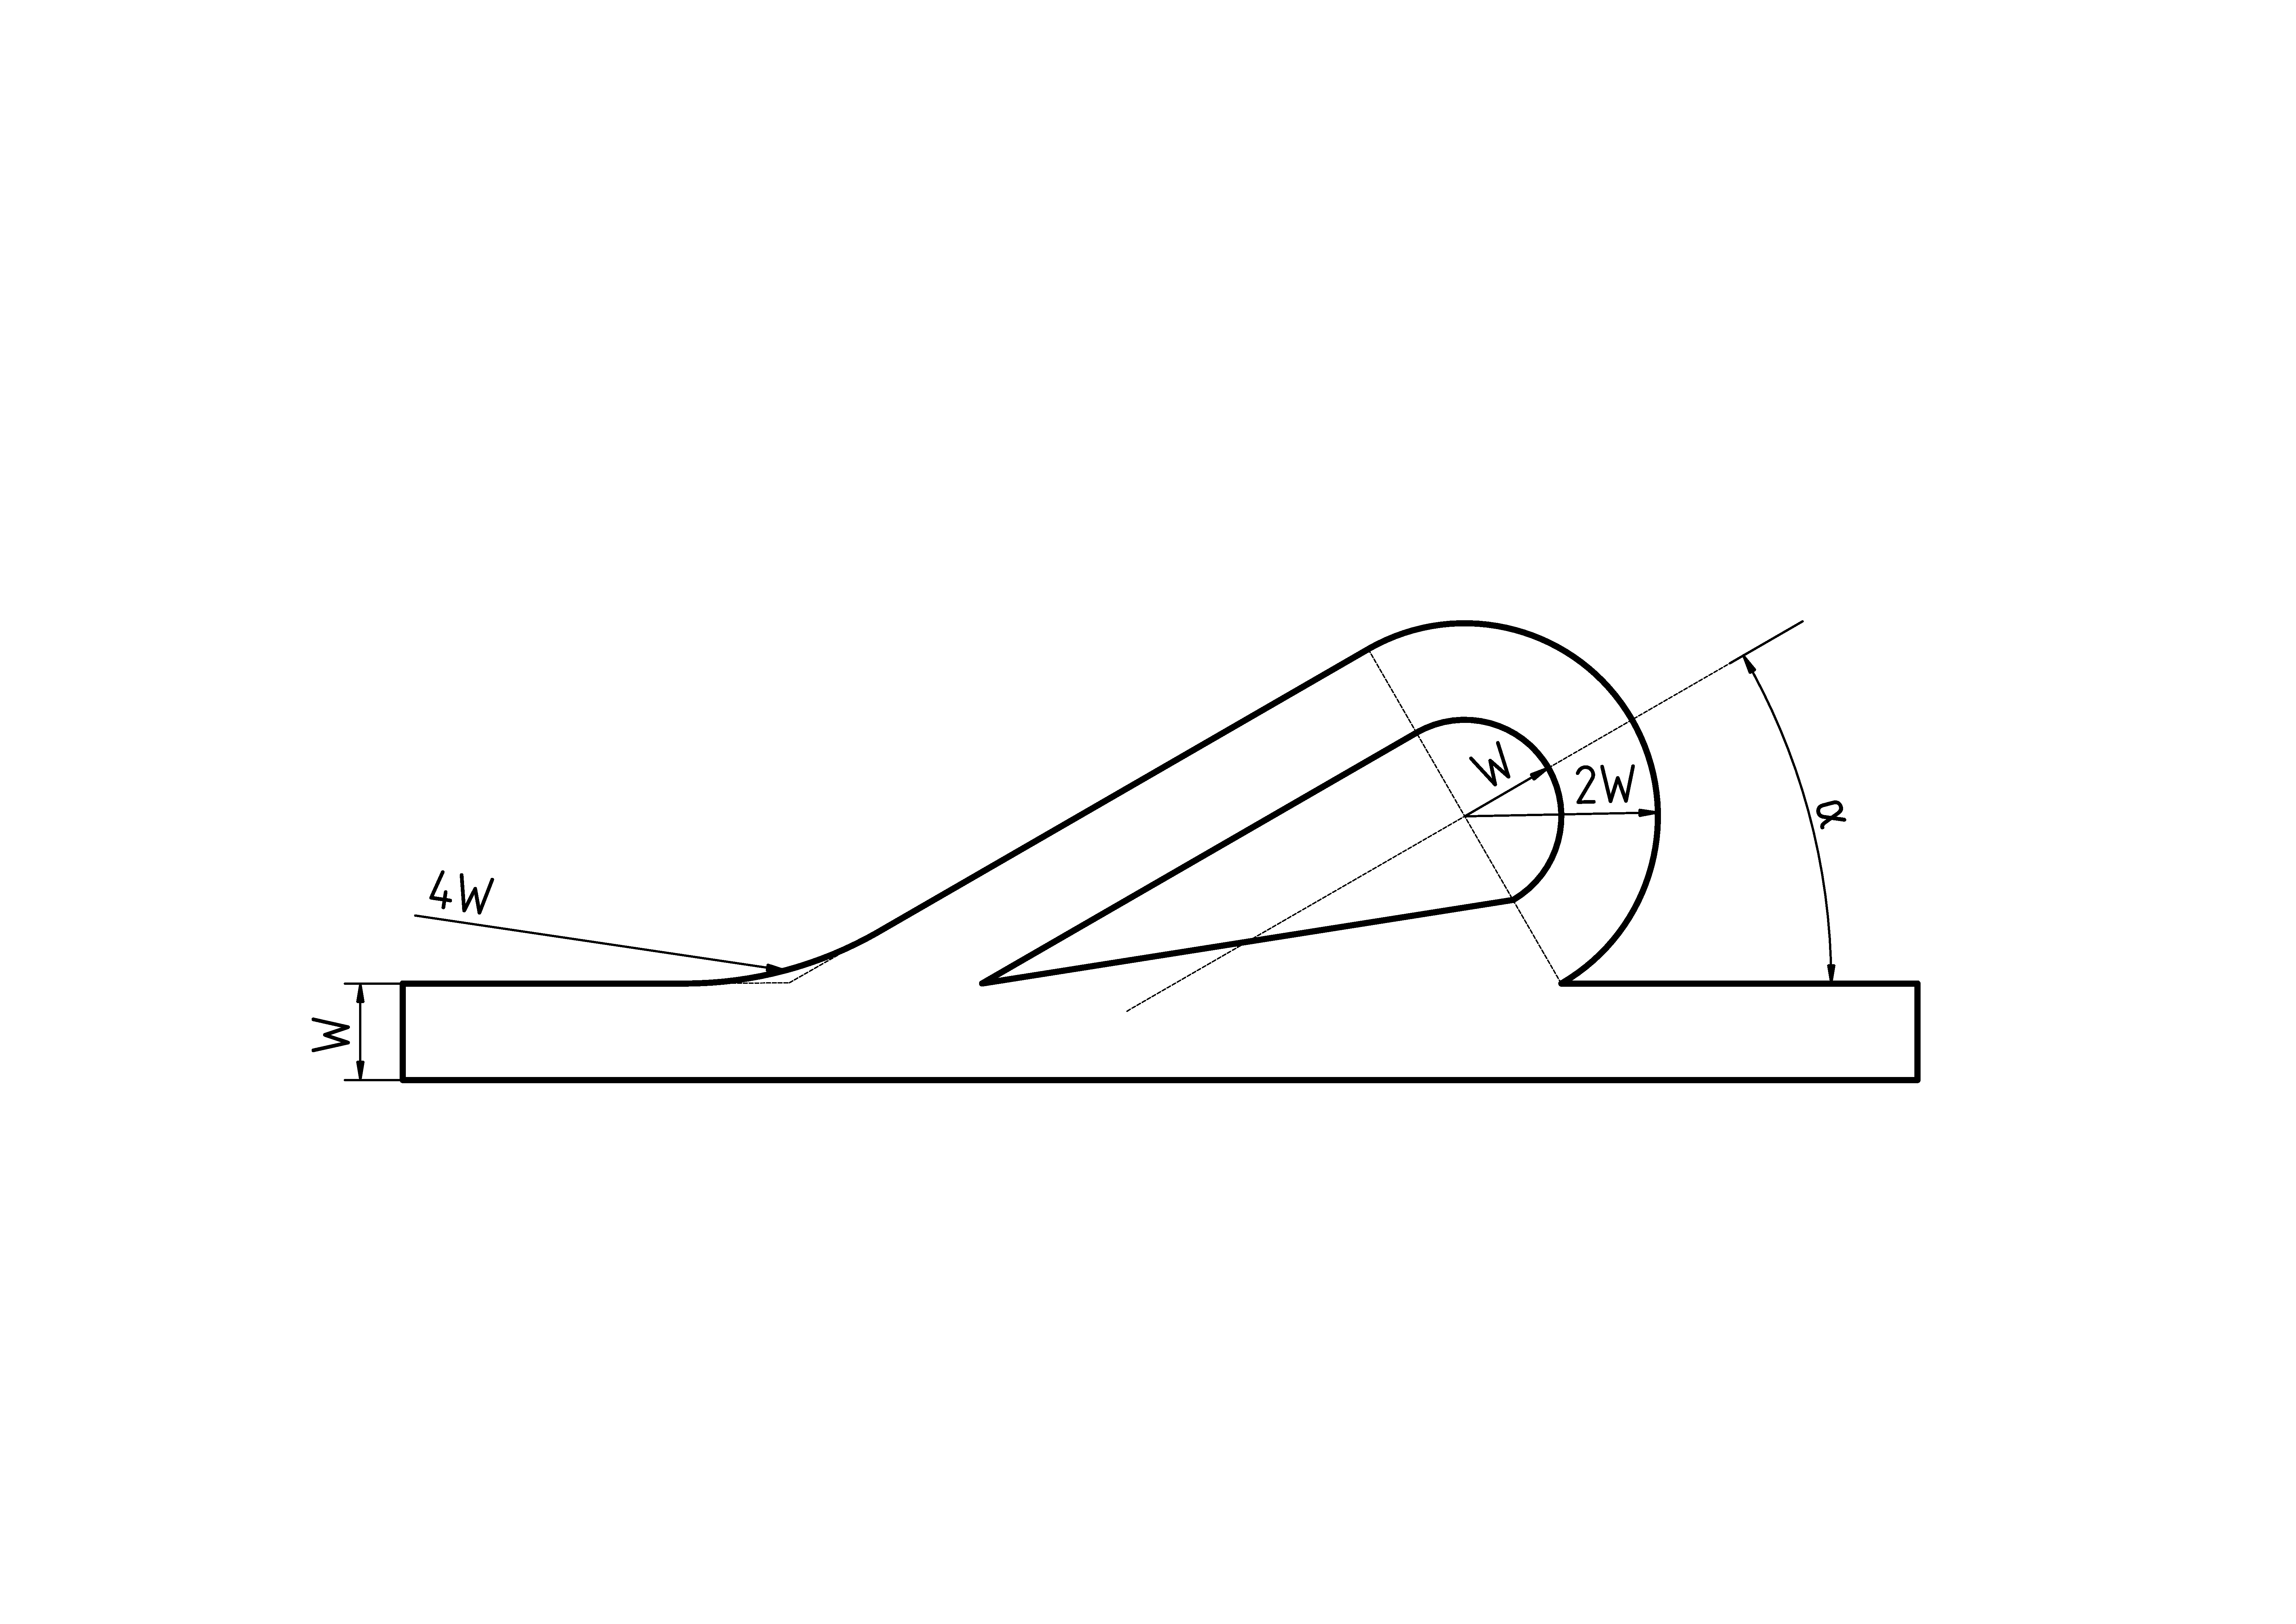
\includegraphics[width = 1\linewidth]{teslaDesign}
        \caption{Клапан Тесла.}
        \label{fig:td}
    \end{figure}
    
    Это прямой канал с U-образным отводным каналом. Задача отводного канала, разделить ток жидкости идущей по основному каналу, и перенаправить отведенную часть против основного потока. Таким образом, клапан Тесла, при обратном подключении и работает, замедляя ток жидкости. Заметным отличием от оригинальной версии клапана Теслы является явно выделенный основной канал, к которому добавлены отводящие каналы.          
    
    На основе выбранного шаблона был написан скрипт на языке Python, для построения параметрической геометрии и расчетной сетки с минимальным количеством независимых параметров. На рис.~\ref{fig:td} схематично показана зависимость геометрии клапана от вводимых параметров, всего независимых параметров два - это ширина канала, W, и угол наклона отводящего канала, $ \alpha  $. Скругление на входе в отводящий канал влияет на эффективность клапана, увеличивая площадь входа в U - образный канал. Основной параметр для параметрического исследования -- это угол $ \alpha  $, а для исследования сеточной сходимости -- это максимальный характерный размер одной ячейки сетки, в микрометрах, при сохранении отношения между минимальным и максимальным размером ячеек.
    
%    \begin{figure}[H]
%        \centering
%        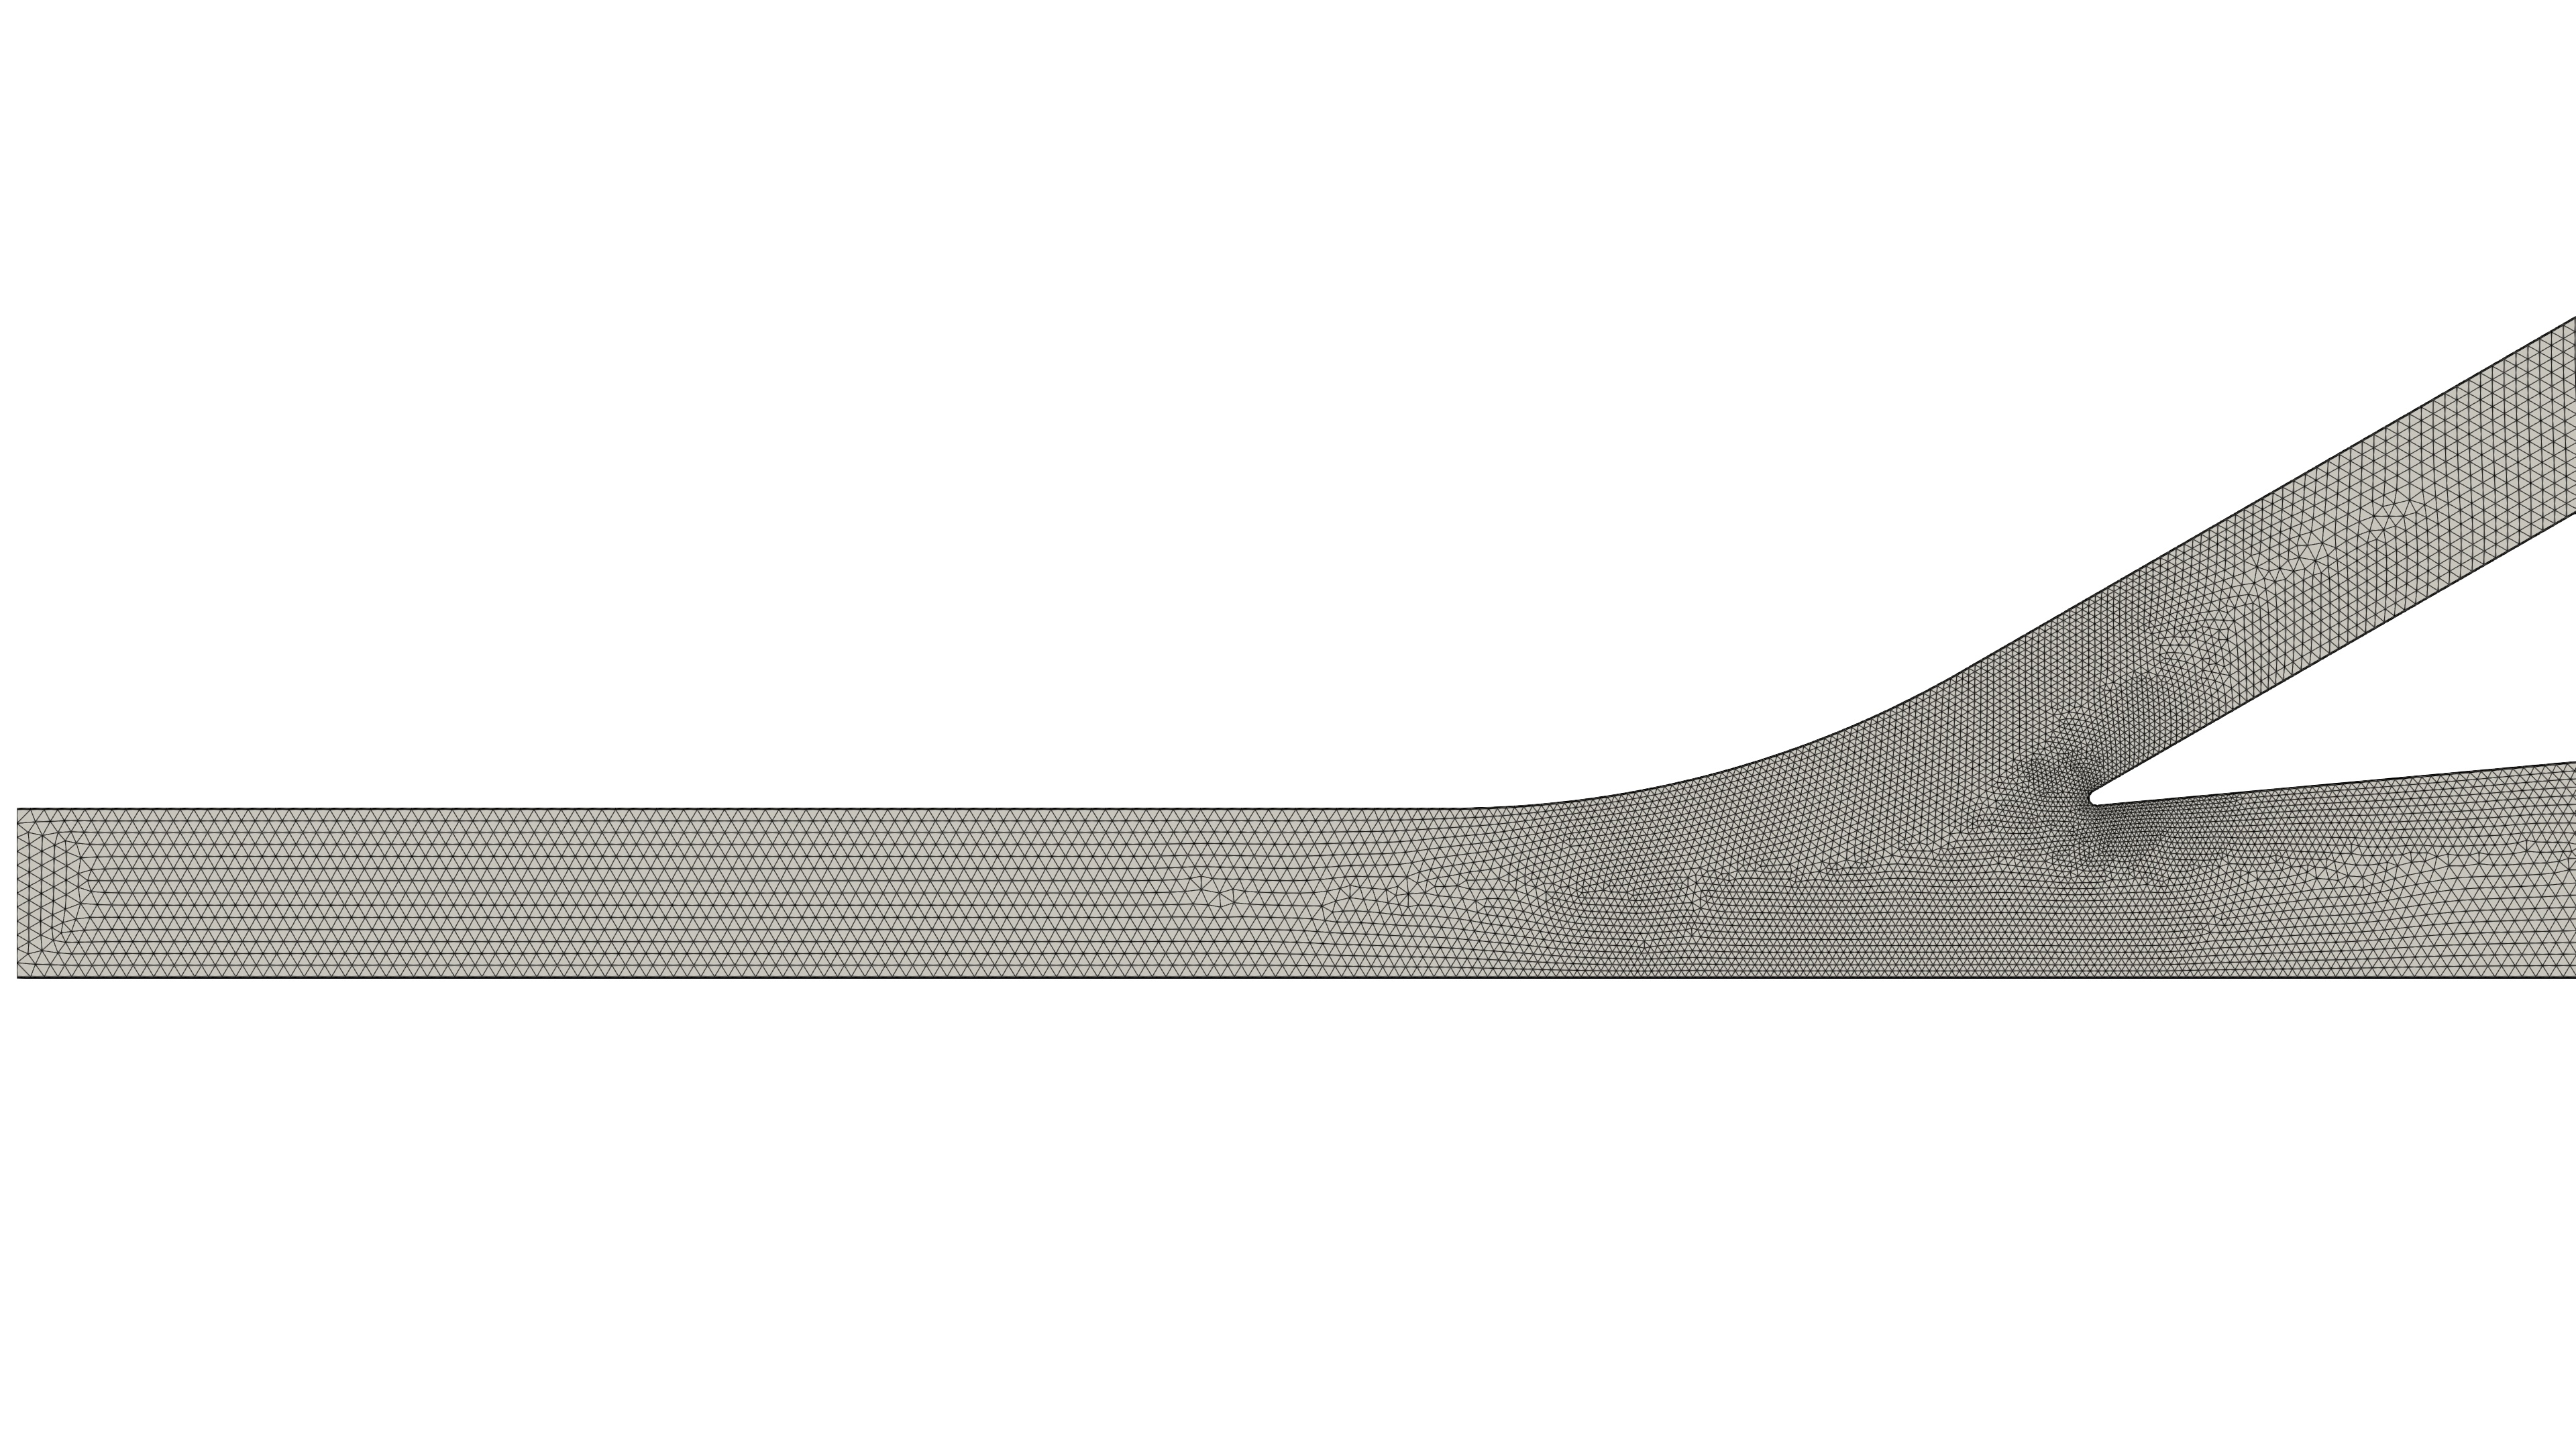
\includegraphics[width = 1\linewidth]{teslaMesh1}
%        \caption{Расчетная сетка.}
%        \label{fig:teslaMesh}
%    \end{figure}
    
    На рис.~\ref{fig:teslaMesh2} угол $\alpha$ равен 30 градусам, ширина канала была выбрана равной 500 мкм или 0.0005 м. Также, можно видеть, что сетка не однородная. В нашей задаче основной интерес сосредоточен в областях, где поток разделяется и перемешивается. В них могут происходить отрывы или скачки, для разрешения градиентов давления и более точного определения профиля скорости разрешение сетки в этих областях выше.
    
    \begin{figure}[H]
        \centering
        \includegraphics[width = 0.7\linewidth]{meshWithZoom}
        \caption{Расчетная сетка.}
        \label{fig:teslaMesh2}
    \end{figure}   
    
    Для разрешения градиента скорости вблизи стенок был добавлен сеточный подслой. Скругления острых углов сделано с целью построения более качественной сетки, радиус скругления фиксирован.
    
    \section{Режим течения и расчет}        
    
    Чтобы определить какого рода перед нами течение, можно рассчитать число Рейнольдса, Re. Исходя из полученного значения, можно будет сделать выводы о характере потока, турбулентное или ламинарное.
    Так как канал нашей конфигурации клапана Теслы имеет квадратное сечение, то формула для определения числа Рейнольдса имеет вид:
    
    \begin{equation}\label{eqn:Re}
        Re = \frac{u D_{H}}{\nu},
    \end{equation}            
    где  u - скорость в канале, м/с, $ D_{H} = \frac{4A}{P} $ - гидравлический диаметр, м, $\nu$ - кинематическая вязкость, м$^{2}/$с. 
    где A - площадь поперечного сечения канала, м$^{2}$, P - смоченный периметр. 
    
    Для нашей конфигурации была выбрана скорость, задаваемая на входе, равной 3 м/с, а число соответственно равно Рейнольдса - 1500.
    
    OpenFoam - это открытый программный комплекс для решения задач механики сплошной среды. SimpleFoam - это стационарный решатель для несжимаемого турбулентного потока, использующий алгоритм SIMPLE. Математическая модель, реализованная в решателе SimpleFoam, имеет вид:
    
    \begin{equation}\label{eqn:simpleFoam}
        \bm{\nabla} \cdot \bm{u} = 0
    \end{equation} 
    
    \begin{equation}\label{eqn:simpleFoam2}
        \bm{\nabla} \cdot \bm{u} \otimes \bm{u} = -\bm{\nabla} p + \bm{\nabla} \cdot \bm{\tau}
    \end{equation} 
    
    Где $\bm{u}$ - скорость, м/с, p - кинематическое давление, м$^{2}/$с$^{2}$, $\bm{\tau}$ - тензор напряжения. 
    Каждый цикл итерации влечет за собой сначала расчет промежуточного поля скорости, которое удовлетворяет линеаризованным уравнениям импульса для предполагаемого распределения давления: затем применяется принцип сохранения массы для настройки скоростей и давлений, так что все уравнения находятся в равновесии.
    
    %       По графику невязок (рис.~\ref{fig:DRLam}) видно, что, при расчете без использования модели турбулентности, решение является неустойчивым. 
    %        
    %        \begin{figure}[H]
        %            \centering
        %            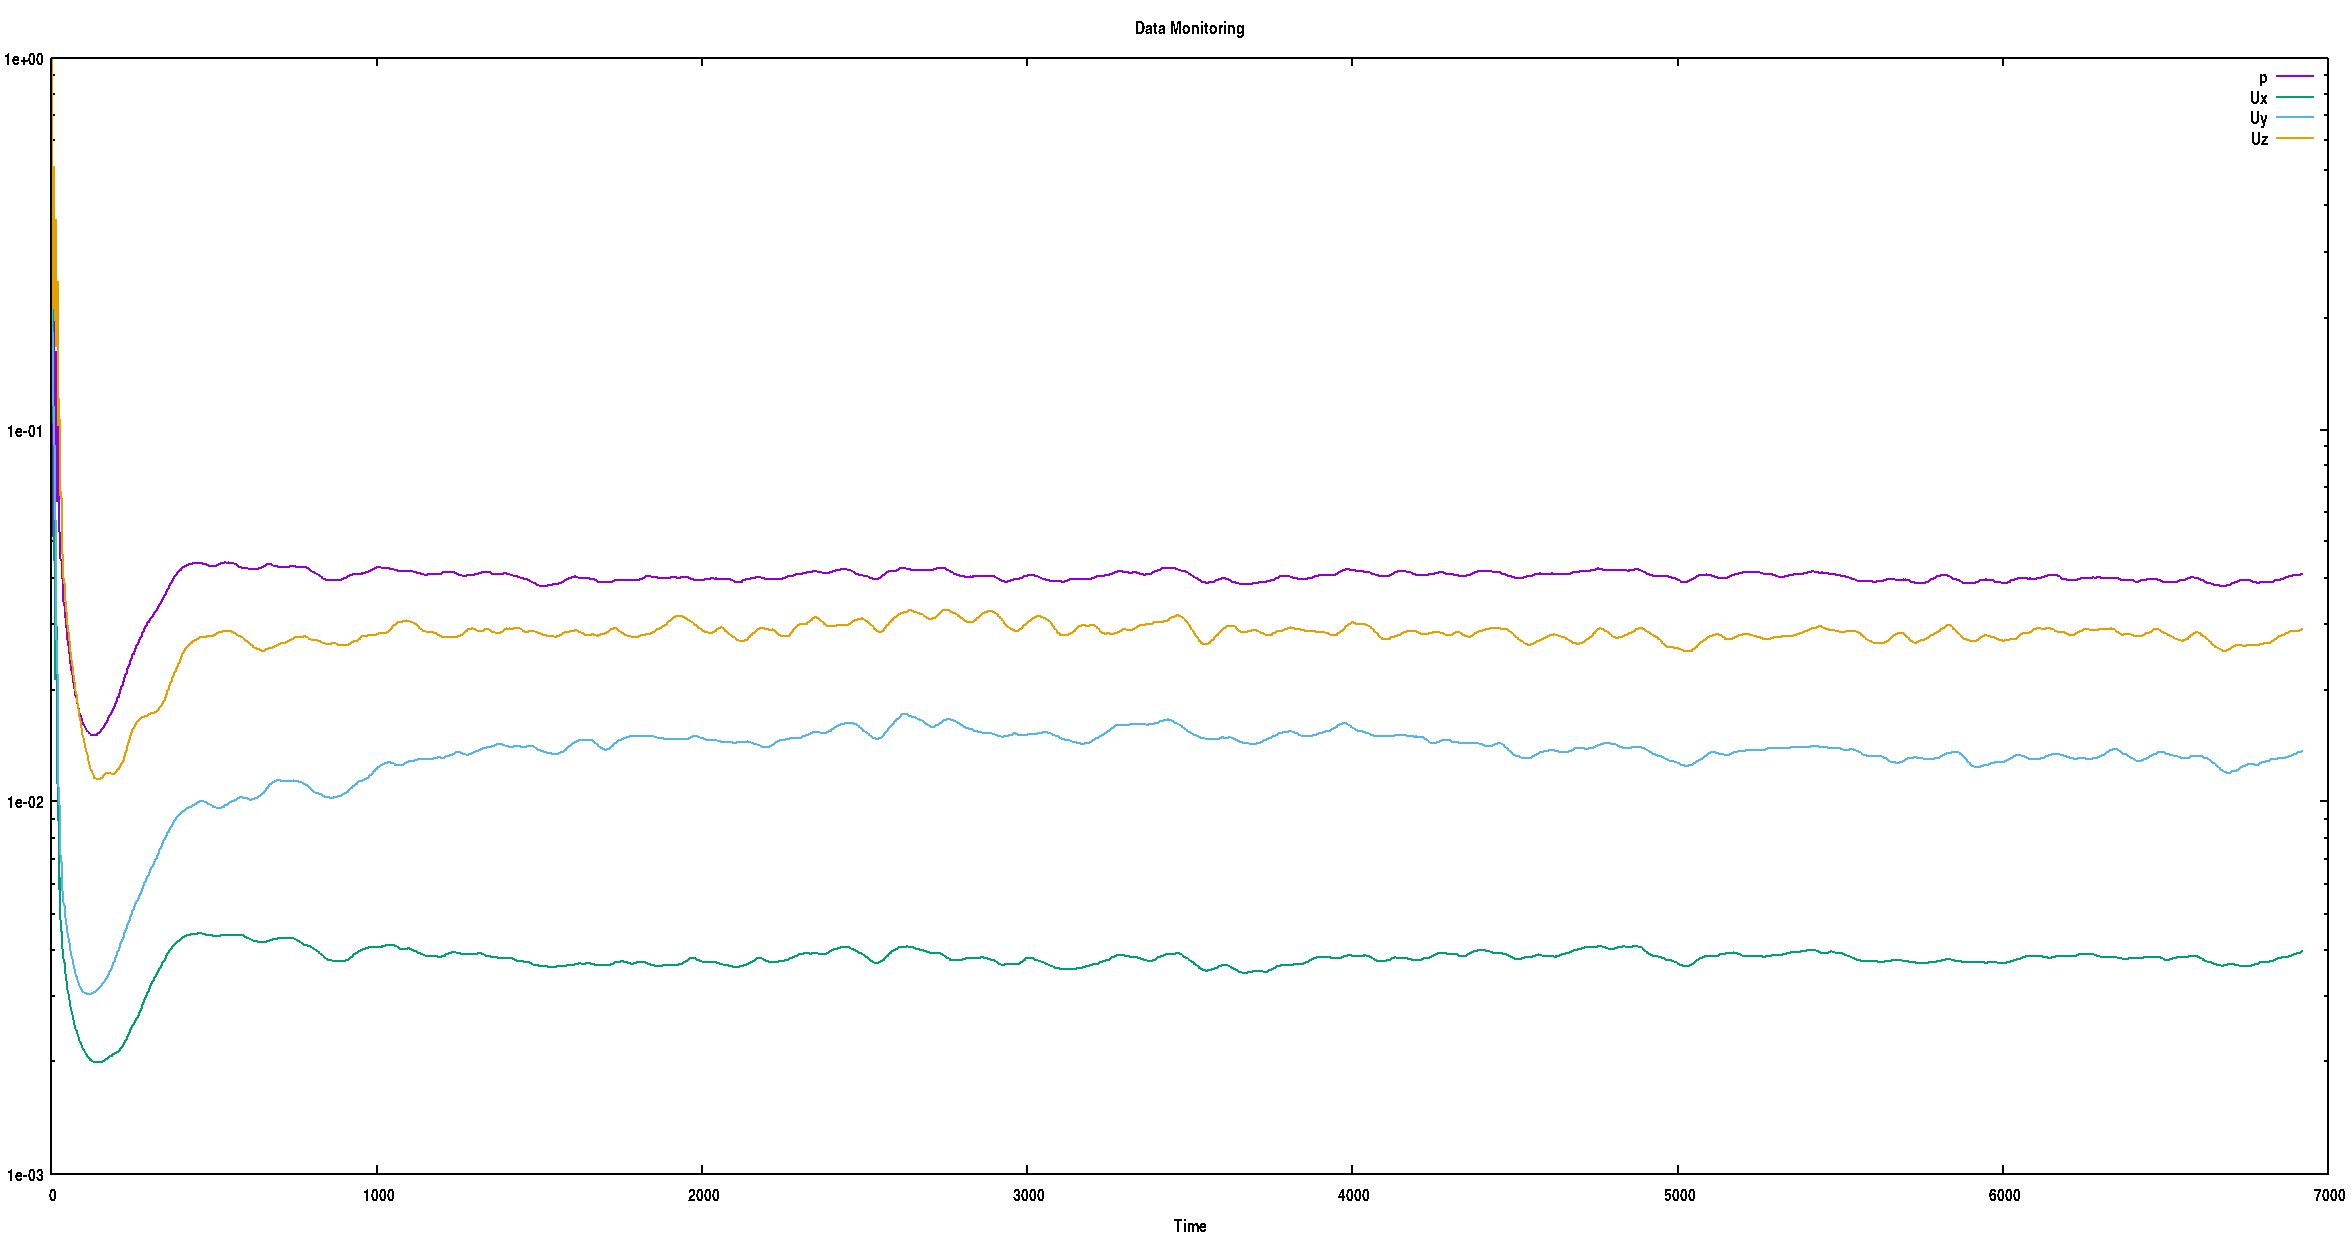
\includegraphics[width = 1\linewidth]{dataMonitoringLaminar}
        %            \caption{Сходимость с ламинарной моделью.}
        %            \label{fig:DRLam}
        %        \end{figure}
    %        
    %        
    %        Исходя из этого было принято решение о подключении турбулентной модели k-epsilon. Выбранным типом моделирования турбулентности был параметр RAS. Модель k-epsilon объединяет уравнения турбулентной кинетической энергии (\ref{eqn:k}), k, и уравнение скорости рассеивания турбулентной кинетической энергии (\ref{eqn:e}), $\epsilon$.
    
    Выбранным типом моделирования турбулентности был параметр RAS. Модель k-epsilon объединяет уравнения турбулентной кинетической энергии (\ref{eqn:k}), k, и уравнение скорости рассеивания турбулентной кинетической энергии (\ref{eqn:e}), $\epsilon$.
    
    \begin{equation}\label{eqn:k}
        \frac{D}{D_{t}}(\rho k) = \nabla \cdot (\rho D_{k}\nabla k) + P - \rho\epsilon
    \end{equation} 
    
    \begin{equation}\label{eqn:e}
        \frac{D}{D_{t}}(\rho\epsilon) = \nabla \cdot (\rho D_{\epsilon}\nabla\epsilon) + \frac{C_{1}\epsilon}{k}(P + C_{3}\frac{2}{3}k\nabla \cdot \bm{u}) - C_{2}\rho\frac{\epsilon^2}{k}
    \end{equation} 
    Где k --- турбулентная кинетическая энергия, м$^2$/с$^2$, $D_{k}$ - Эффективная диффузионная способность для k, P - скорость производства турбулентной кинетической энергии, м$^2$/с$^-3$, $\epsilon$ - скорость рассеивания турбулентной кинетической энергии, м$^2$/с$^-3$, $D_{\epsilon}$ - Эффективная диффузионная способность для $\epsilon$.
    
    Далее решается уравнение для турбулентной вязкости:
    
    \begin{equation}\label{eqn:mu}
        \nu_{t} = C_{\mu}\frac{k^2}{\epsilon}
    \end{equation} 
    Где $C_{\mu}$ - модельный коэффициент турбулентной вязкости, $\mu_{t}$ - турбулентная вязкость, м$^2$/с$^-1$.
    
    %        В результате, мы видим, что график невязок, при подключенной модели турбулентности k-epsilon, показывает нам устойчивое решение (рис.~\ref{fig:DRRAS}).  
    %        
    %        \begin{figure}[H]
        %            \centering
        %            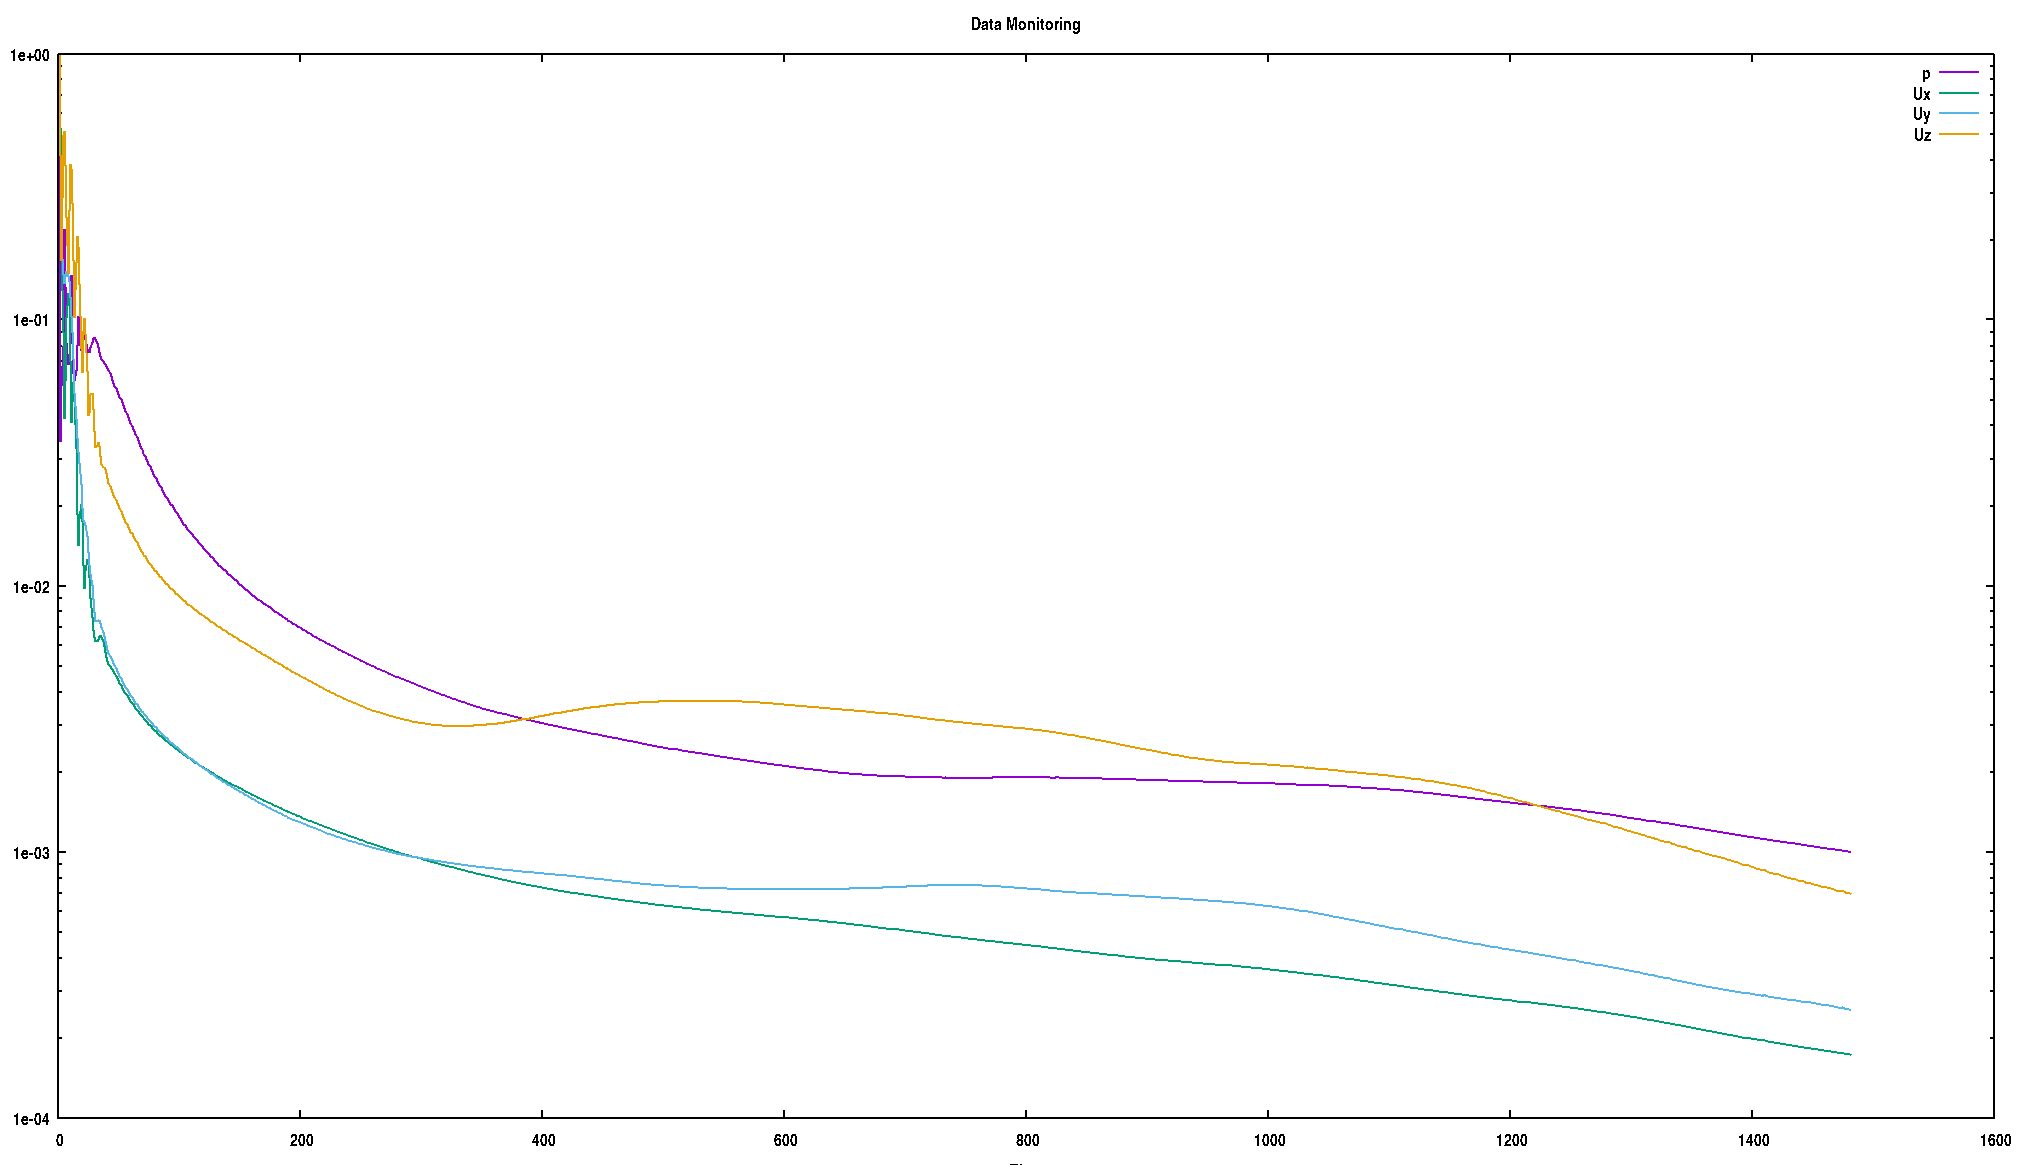
\includegraphics[width = 1\linewidth]{dataMonitoringRAS}
        %            \caption{Сходимость с моделью турбулентности.}
        %            \label{fig:DRRAS}
        %        \end{figure}
    
    Граничные условия для решения уравнений турбулентности заданы через интенсивность для k (\ref{eqn:kI}) и через длину перемешивания для $\epsilon$ (\ref{eqn:el}). Граничные условия для скорости заданы через объемный расход, для давления через абсолютное давление (\ref{eqn:P0}).
    
    \begin{equation}\label{eqn:kI}
        k_{p} = 1.5 (I |U|)^2
    \end{equation}
    Где $k_{p}$ - кинетическая энергия на границе, м$^2$/с$^2$, I - интенсивность турбулентности.
    
    \begin{equation}\label{eqn:el}
        \epsilon_{p} = \frac{C_{\mu}^{0.75} k^{1.5}}{L}           
    \end{equation}
    Где $\epsilon_{p}$ - диссипация кинетической энергии на границе, м$^2$/с$^-3$, L - шкала длины.
    
    \begin{equation}\label{eqn:P0}
        p_{p} = p_{0} + \frac{1}{2}\ \left|u_{0}\right|^2 - \frac{1}{2}\ \left|u\right|^2
    \end{equation}
    Где $p_{p}$ - давление на границе, м$^{2}/$с$^{2}$, $p_{0}$ - внешнее статическое давление, м$^{2}/$с$^{2}$, $u$ - скорость, м/с, $u_{0}$ - внешняя скорость, м/с.\\
    
    Оценить эффективность клапана Теслы, после получения результатов расчета, мы можем, посчитав его диодность, Di (\ref{eqn:Di}). Если Di > 1, то рассматриваемый клапан можно считать рабочим. Для этого мы проводили расчет нашей конфигурации клапана Тесла с одинаковыми параметрами дважды, но при разных подключениях: при обратном, когда перепад давления наибольший, и, при прямом, когда перепад давления наименьший. Полученные данные фиксировались.         
    
    \begin{equation}\label{eqn:Di}
        Di = (\frac{\bigtriangleup p_{r}}{\bigtriangleup p_{f}})_Q
    \end{equation}
    Где $\bigtriangleup p_{r}$ - перепад давления при обратном подключении, $\bigtriangleup p_{f}$ - перепад давления при прямом подключении для скорости потока Q.
    
    \section{Результаты}
    
    При выборе минимального разрешения сетки, мы остановились на таком разрешении, которое позволяло бы на входе поместиться 5 ребрам ячеек расчетной сетки (рис.~\ref{fig:minMesh}). Такое решение было принято в пользу лучшей сходимости задачи.
    
    \begin{figure}[H]
        \centering
        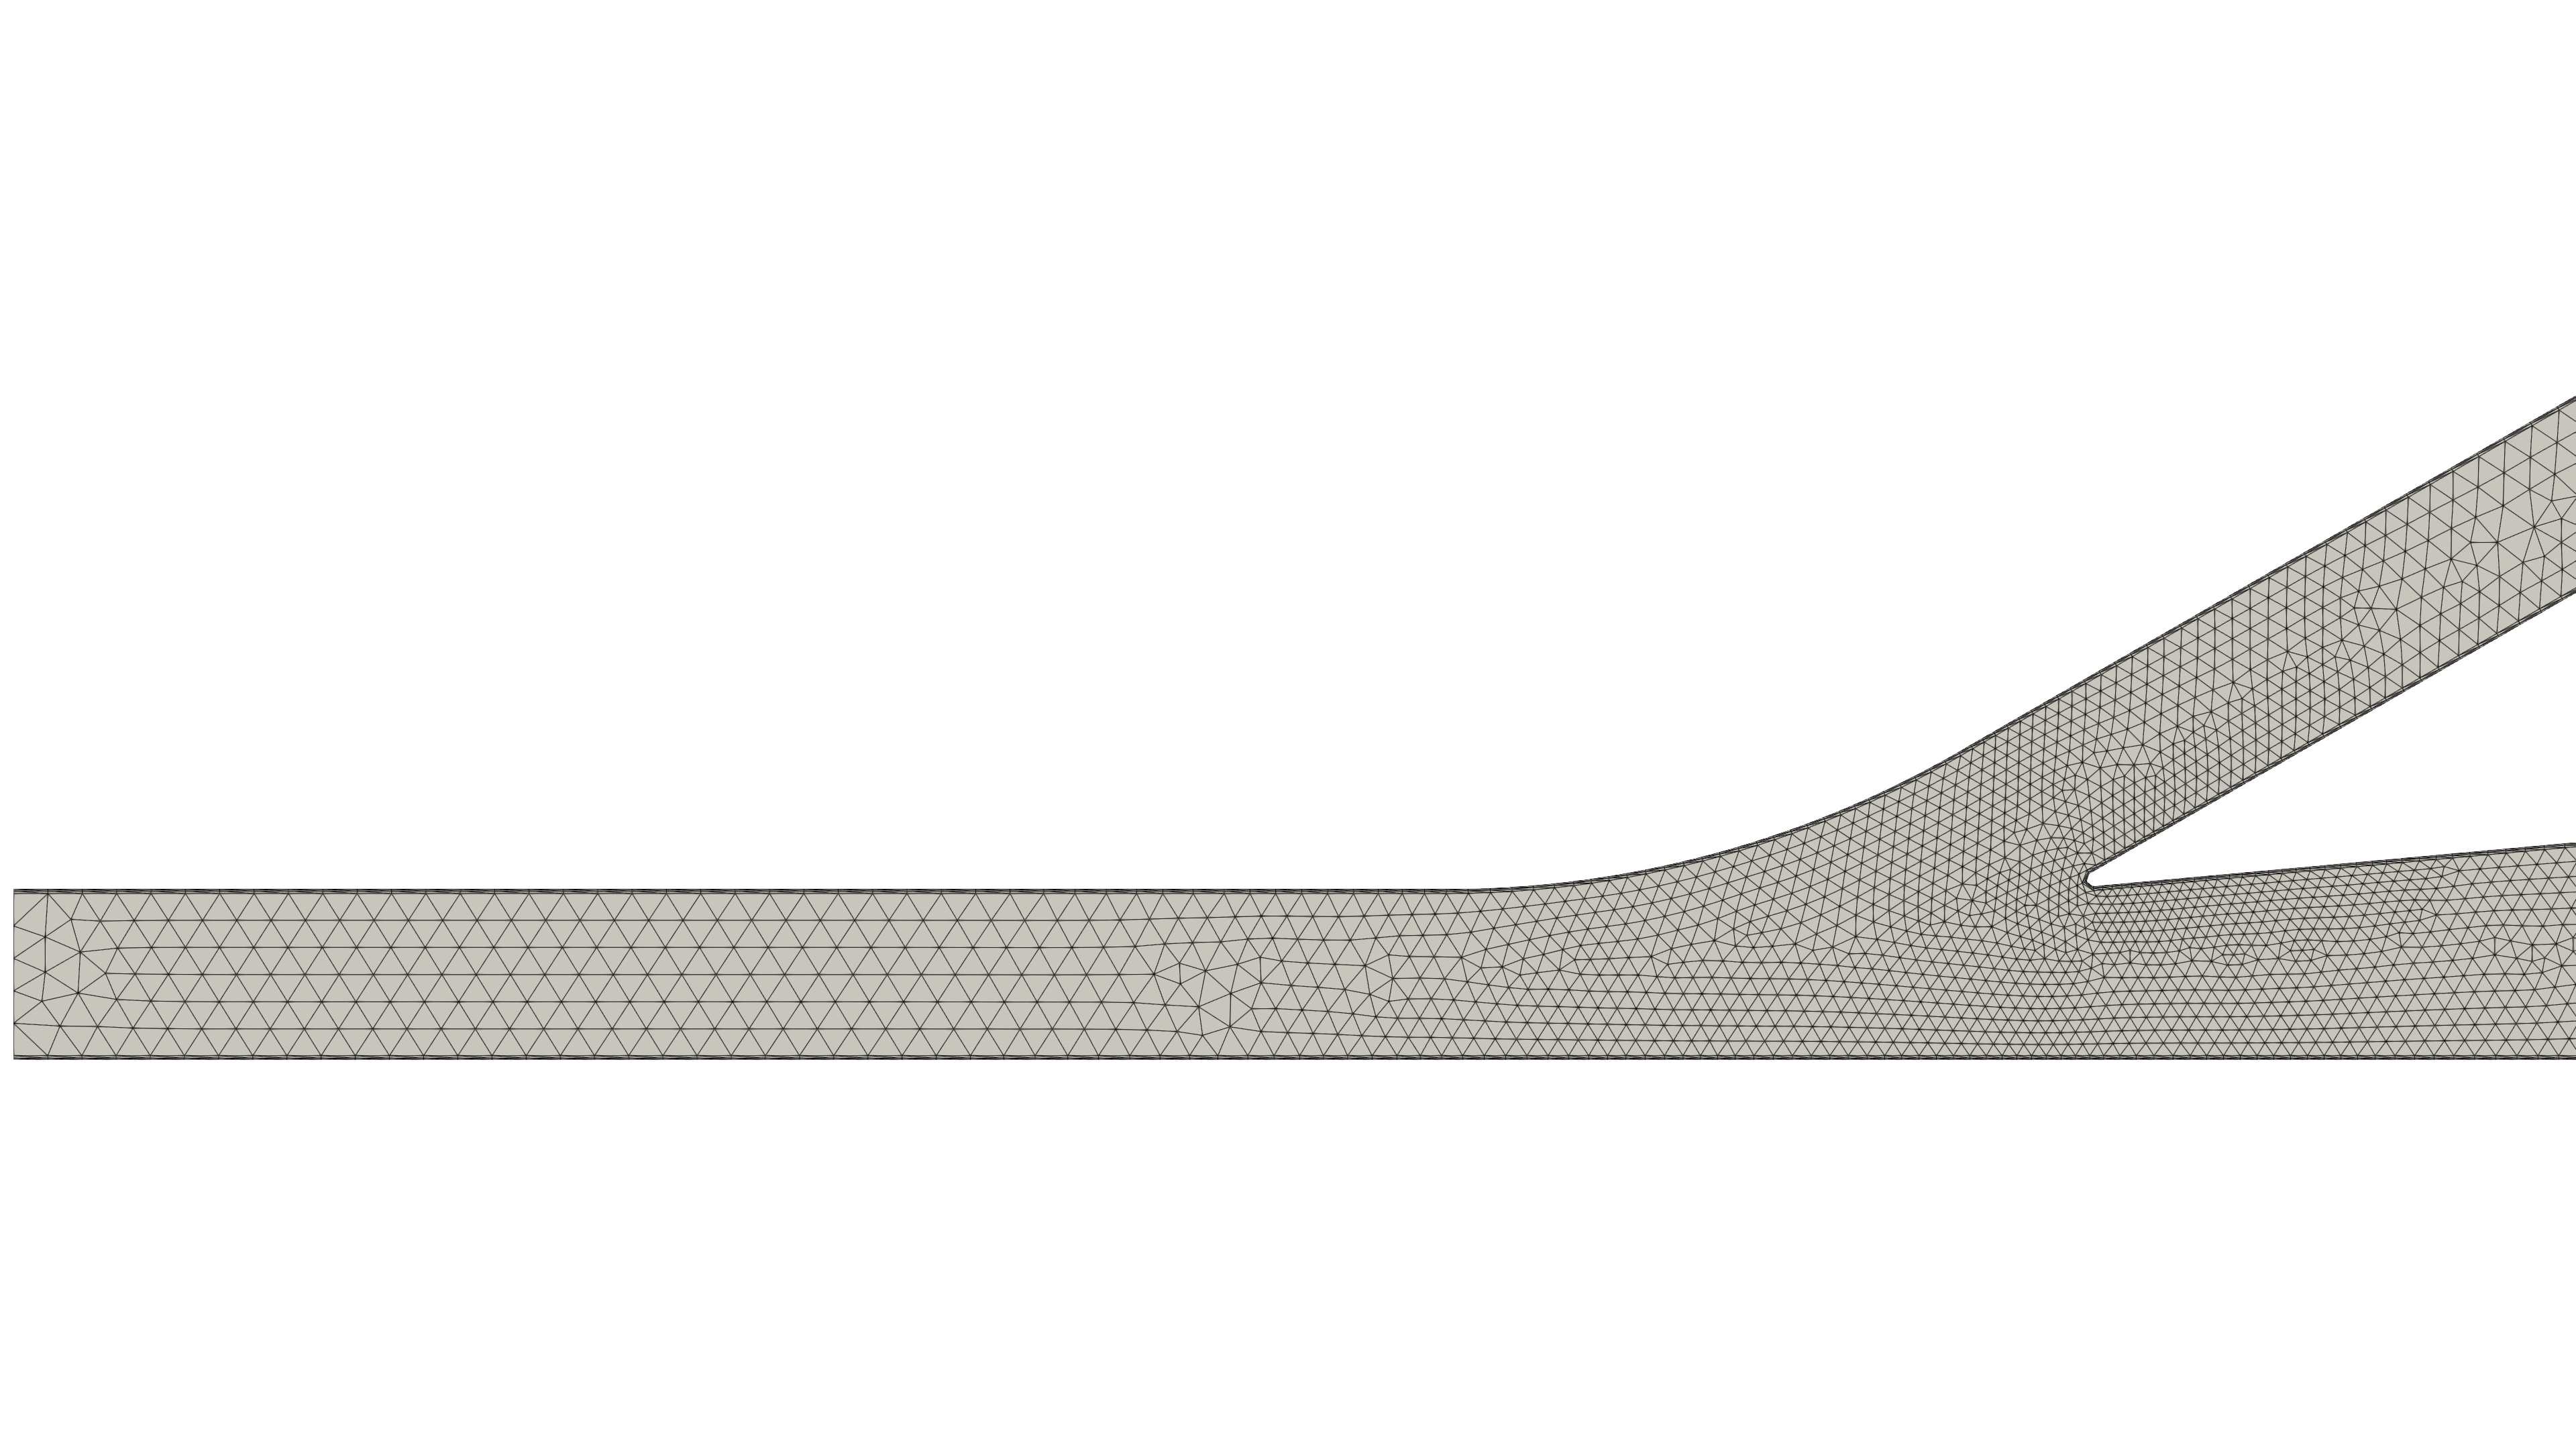
\includegraphics[width = 1\linewidth]{minMesh}
        \caption{Минимальное разрешение сетки.}
        \label{fig:minMesh}
    \end{figure}
    
    Рассмотрим полученные в ходе расчетов поля давления и скорости при обратном подключении (рис.~\ref{fig:UPFieldsReverse}). На изображении поля давления видно, как по мере удаления от входа, давление в клапане снижается и имеет вид приближенный к линейному. Видно, как в местах где поток разделяется и смешивается, происходят скачки давления. Изображение поля скорости, демонстрирует нам значительное падание скорости между участками клапана, где происходит разделение и смешивание потоков жидкости.
    
    \begin{figure}[H]
        \centering
        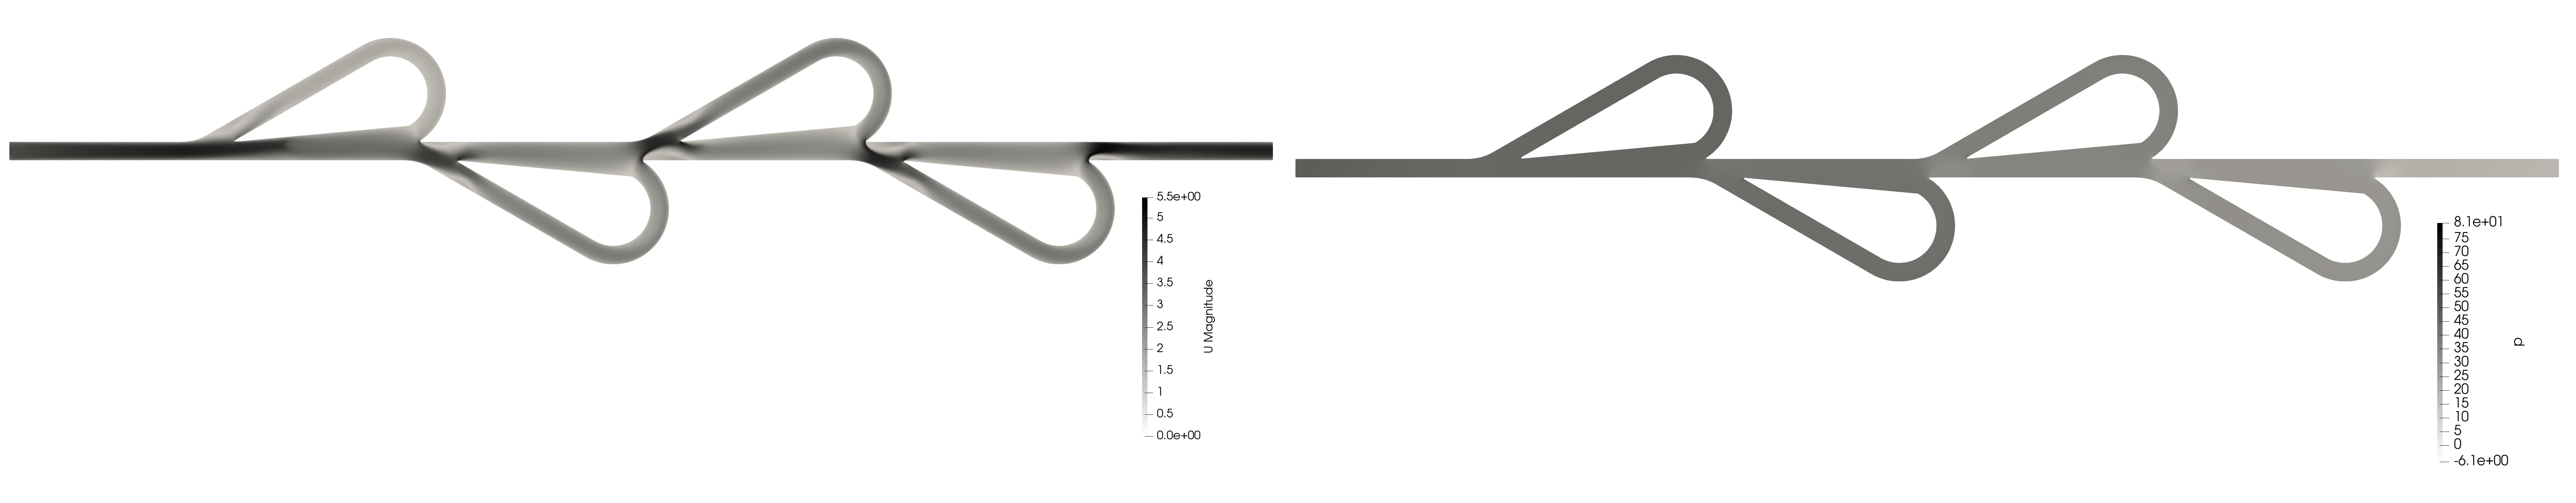
\includegraphics[width = 1\linewidth]{UPFieldsReverse}
        \caption{Поле скорости и давления при обратном подключении.}
        \label{fig:UPFieldsReverse}
    \end{figure}
    
%    \begin{figure}[H]
%        \centering
%        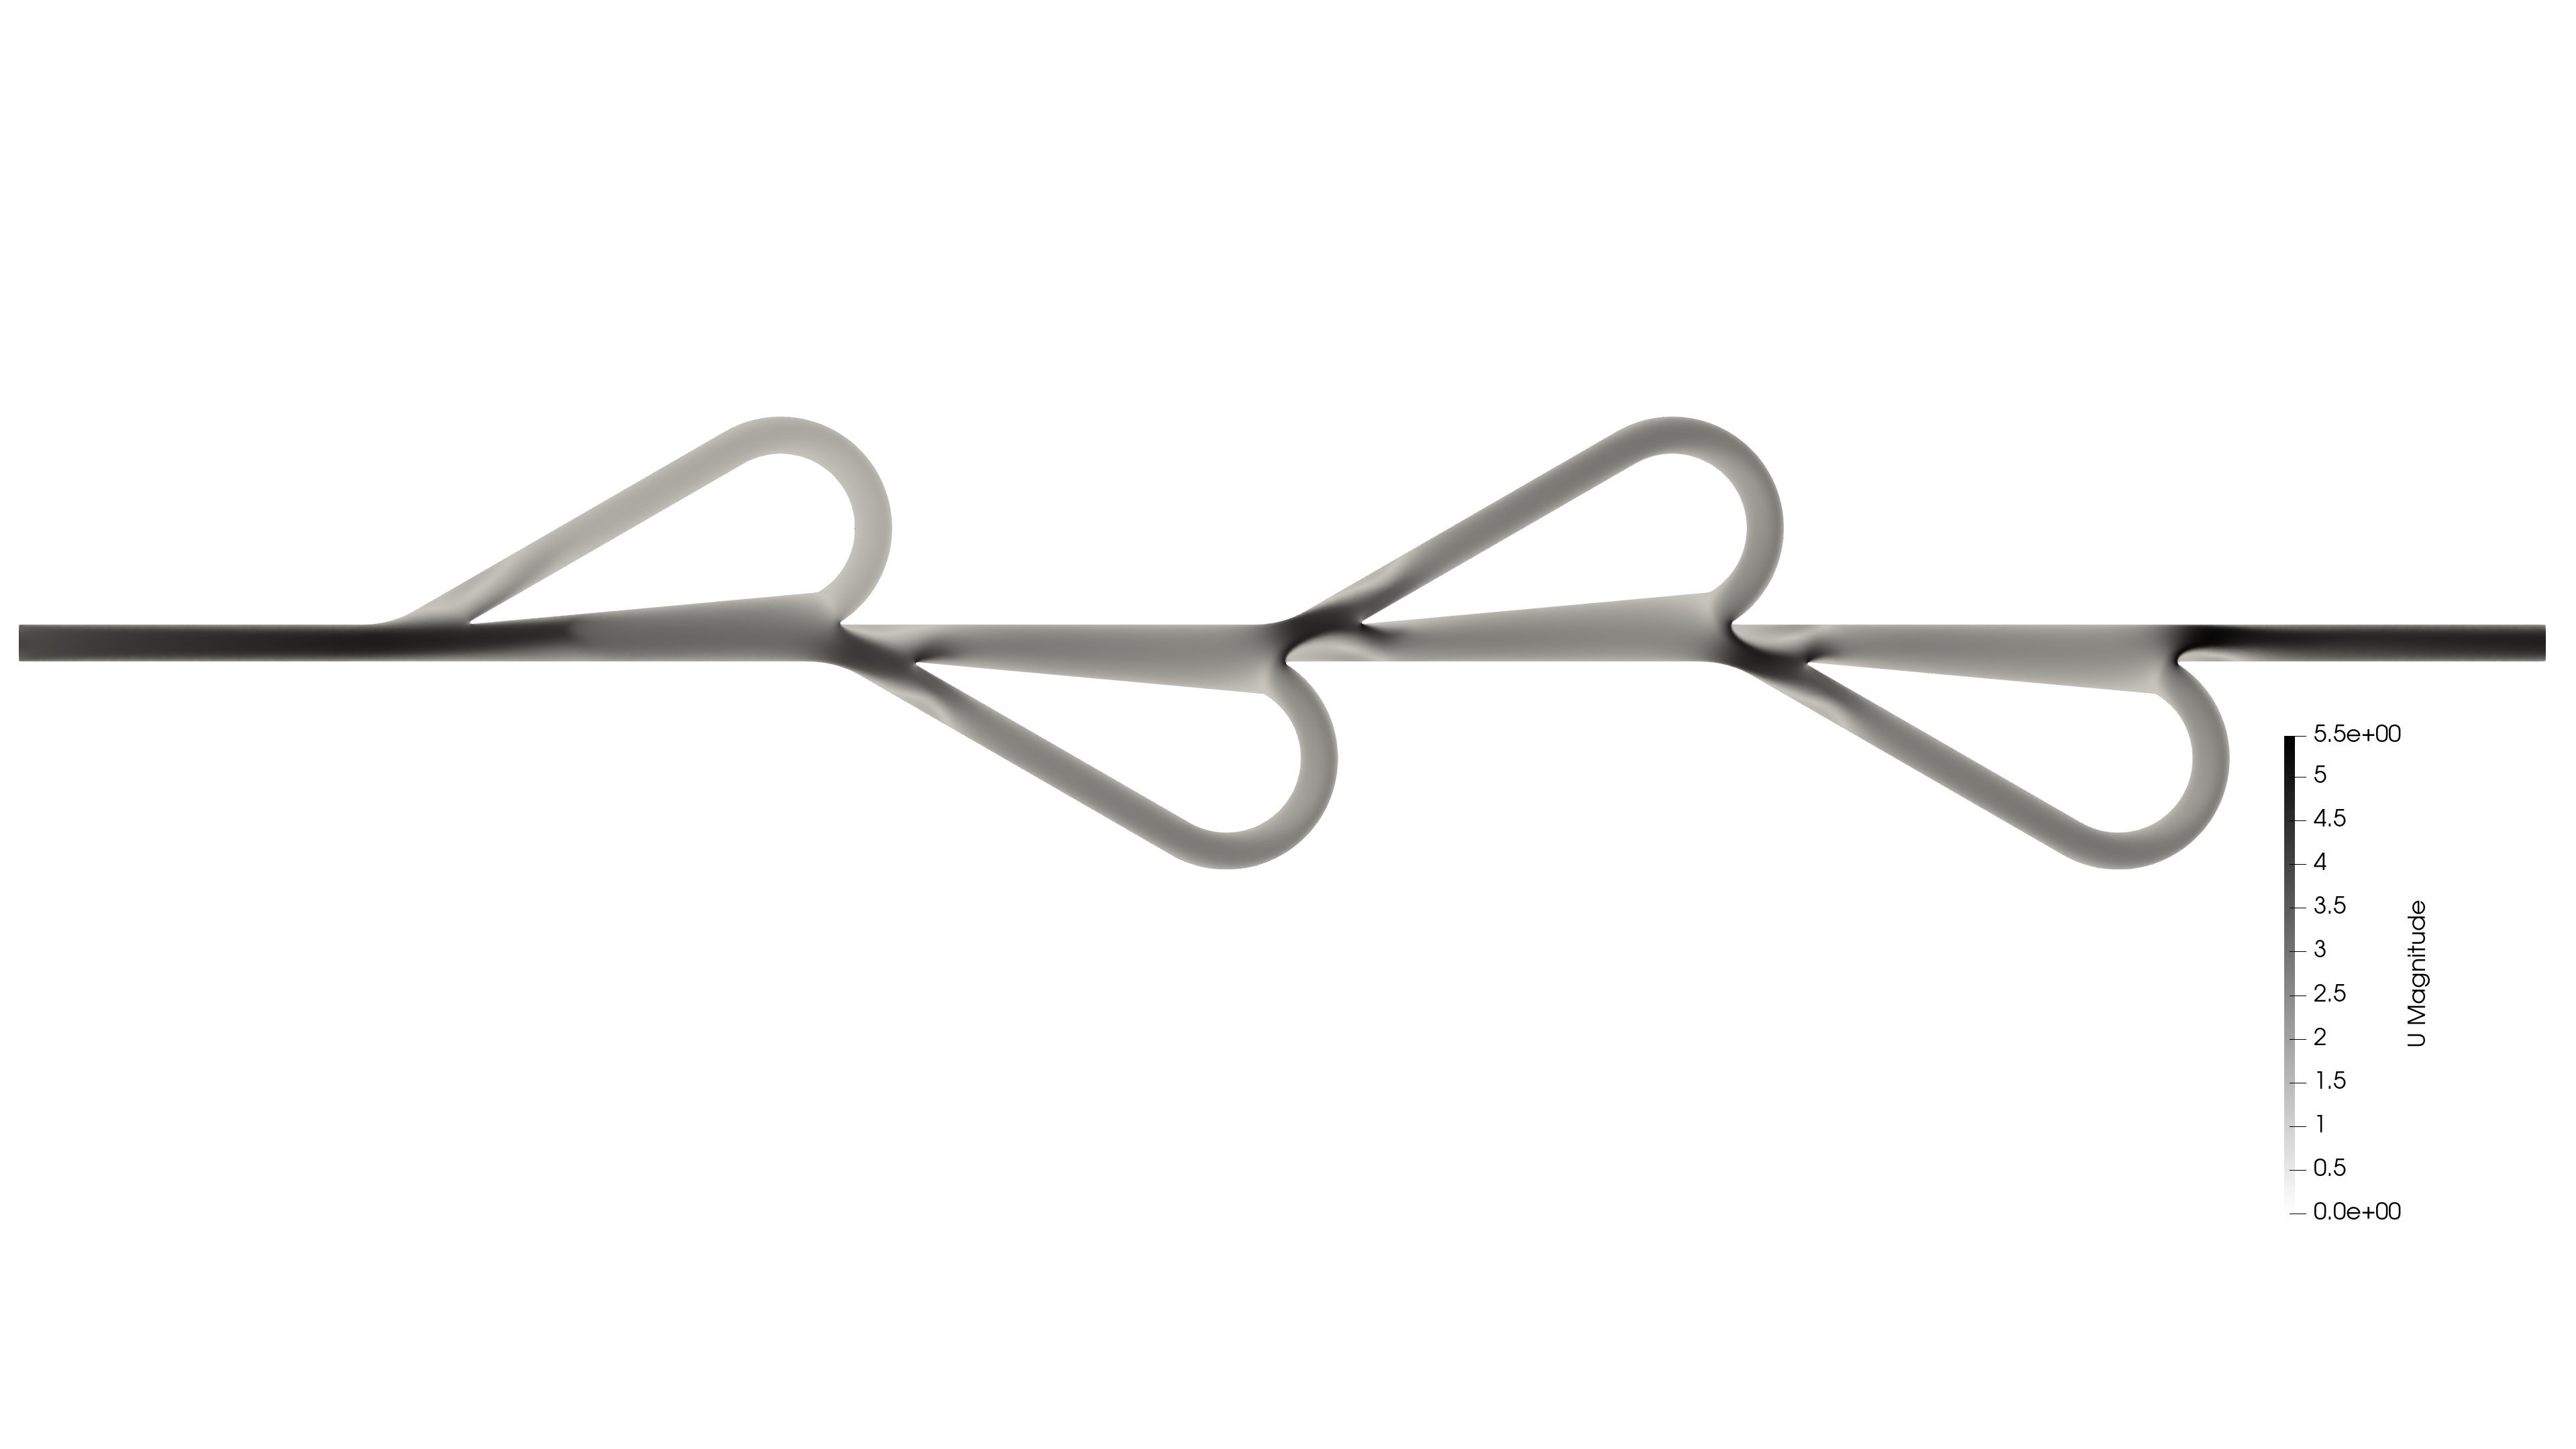
\includegraphics[width = 1\linewidth]{UFieldsReverse}
%        \caption{После скорости при обратном подключении.}
%        \label{fig:UFieldsReverse}
%    \end{figure}
    
    Поле скорости (рис.~\ref{fig:UPFieldsDirect}) при прямом подключении. Видно, как в клапане образуется явно выделенное ядро потока, течение более не рассеивается геометрией клапана так, как это было при обратном подключении. Поле давления линейно, и можно видеть, как отдаляясь от входа клапана, давление падает.
    
    \begin{figure}[H]
        \centering
        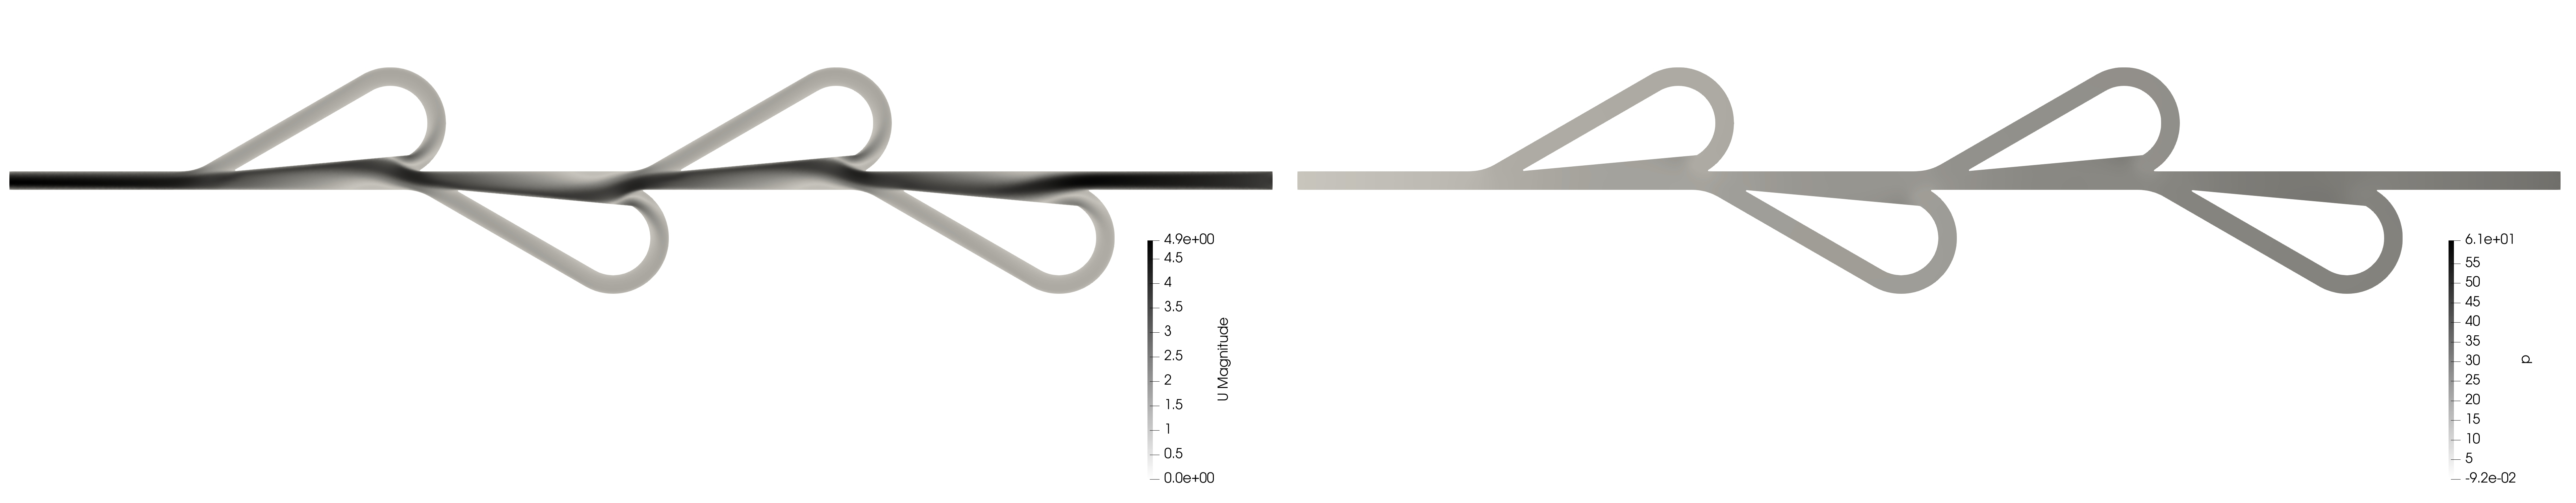
\includegraphics[width = 1\linewidth]{UPFieldsDirect}
        \caption{Поле скорости и давления при прямом подключении.}
        \label{fig:UPFieldsDirect}
    \end{figure}
    
%    \begin{figure}[H]
%        \centering
%        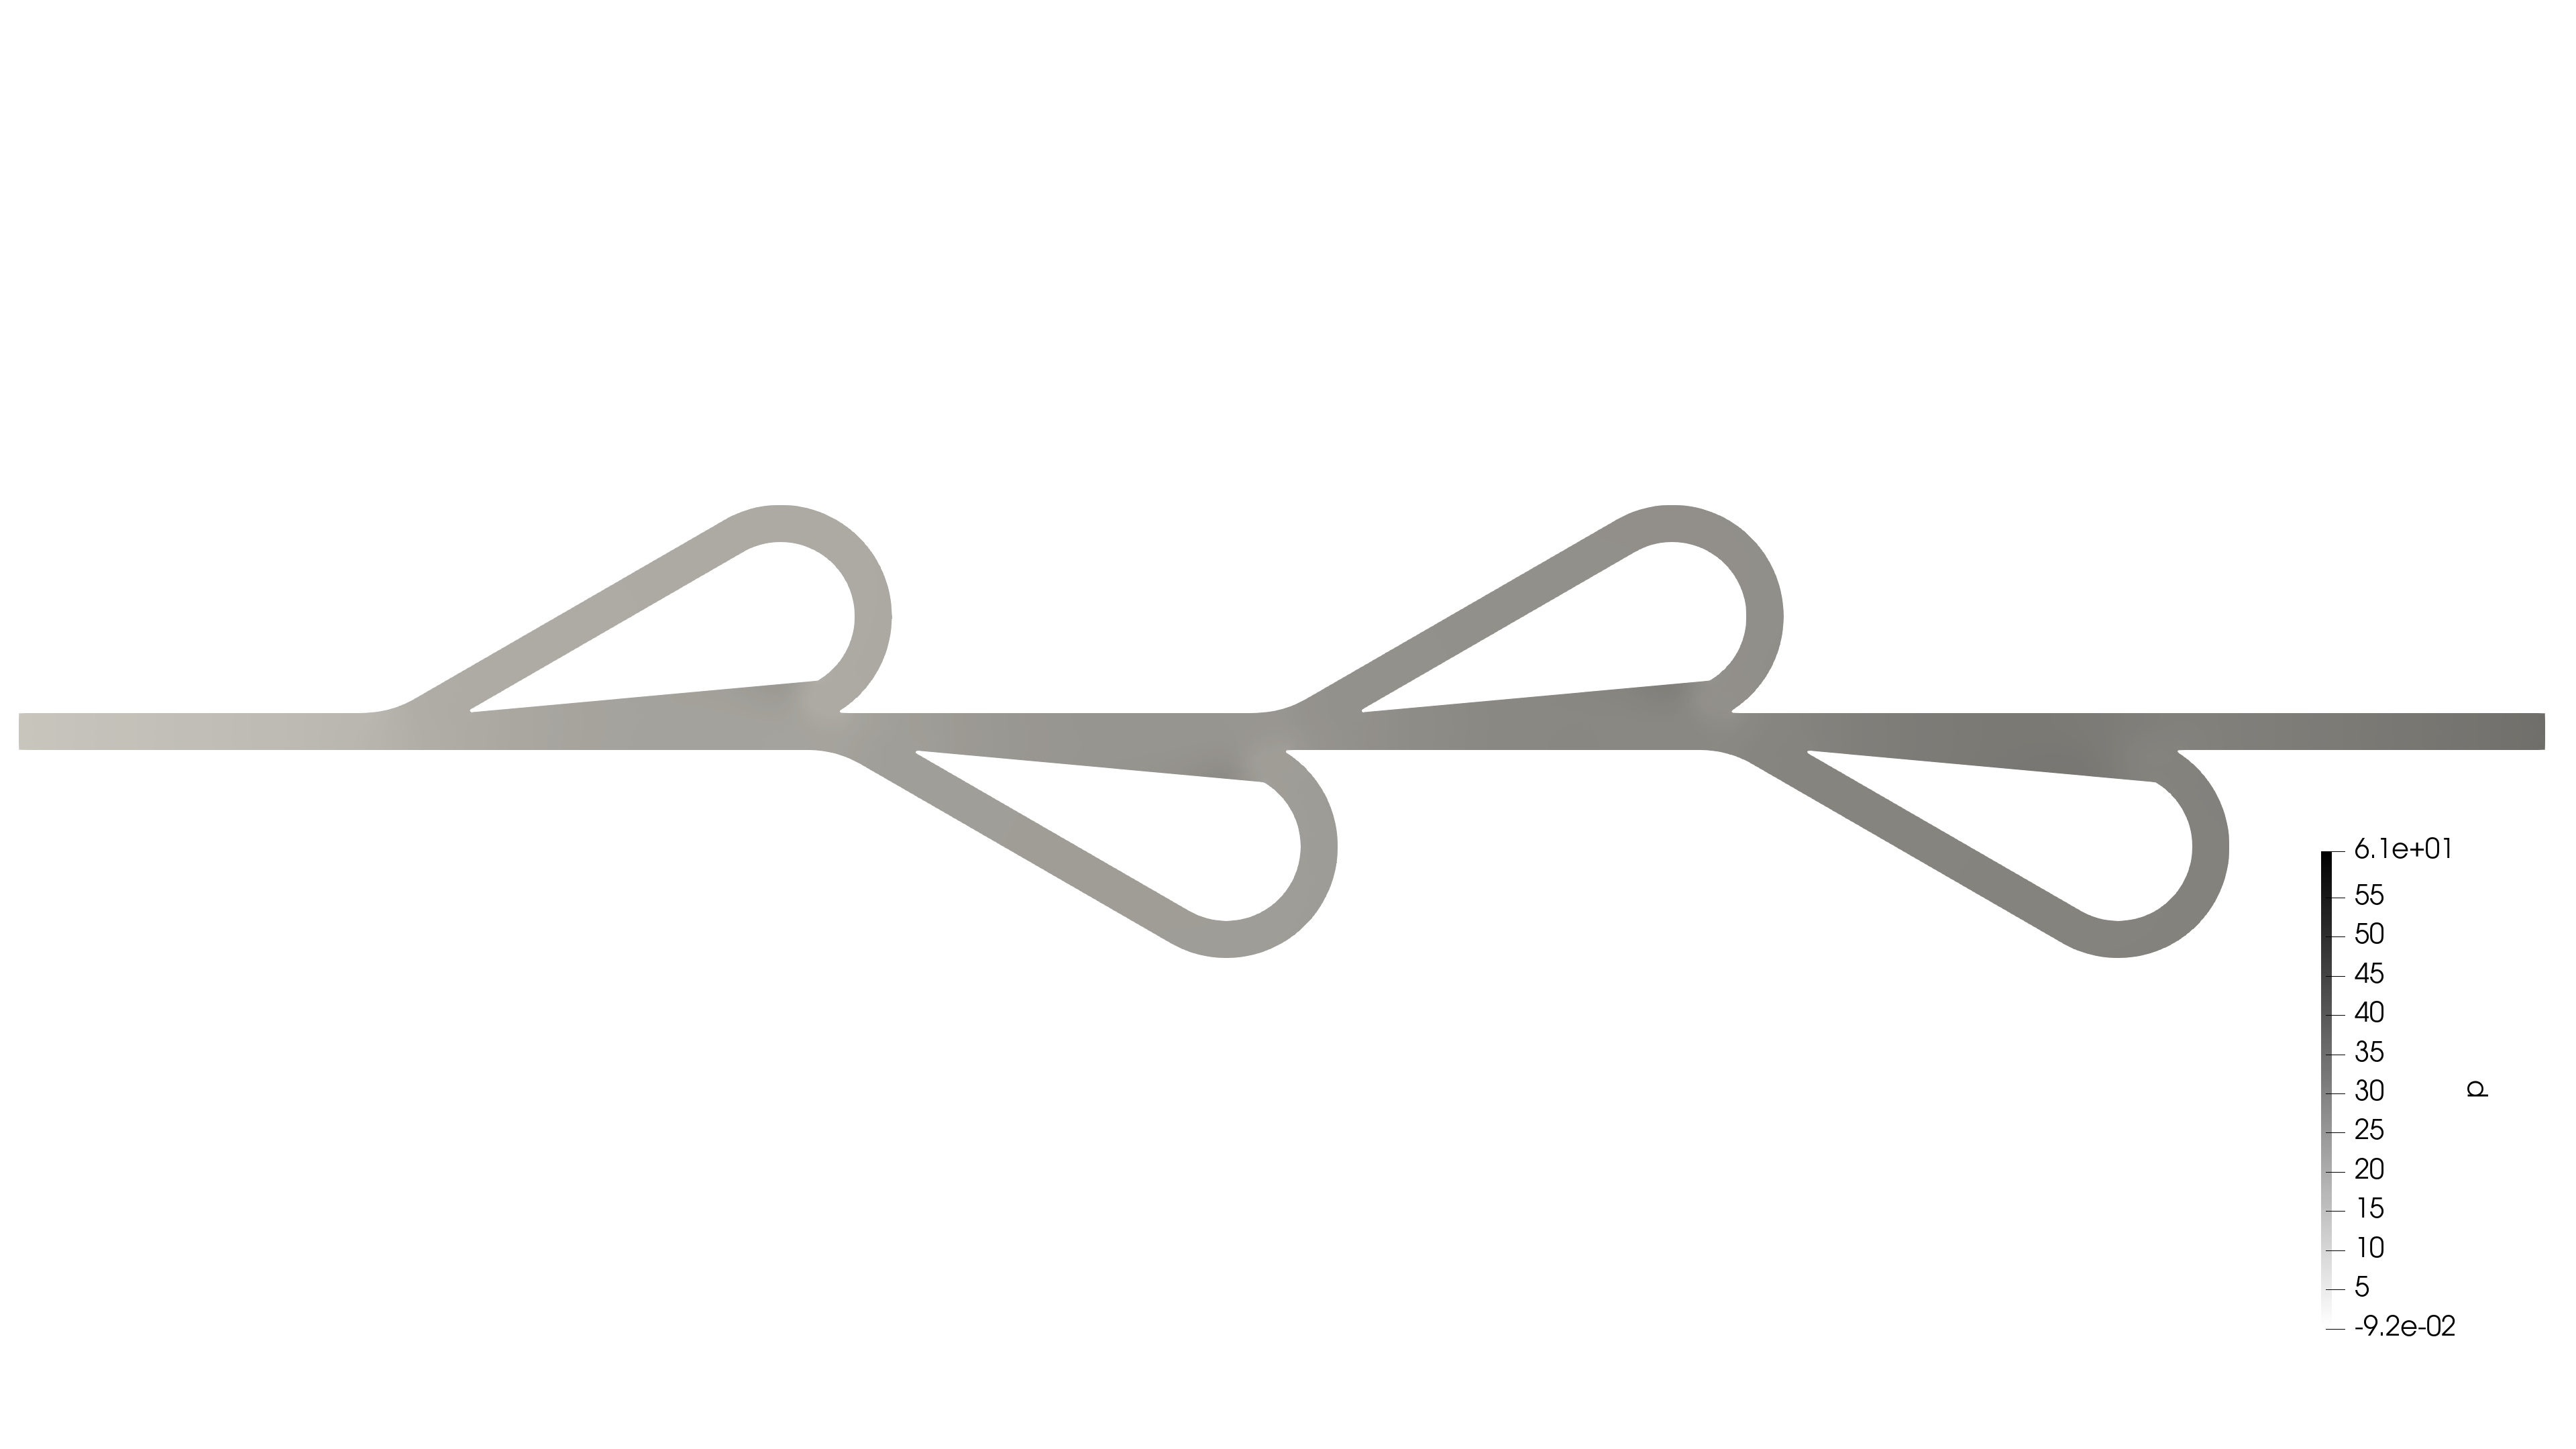
\includegraphics[width = 1\linewidth]{PFieldsDirect}
%        \caption{После давления при прямом подключении.}
%        \label{fig:PFieldsDirect}
%    \end{figure}    
    
    Ход исследования сеточной сходимости. Было принято решение отталкиваться от максимального размера ячейки. Каждая следующая сетка отличалась от предыдущей тем, что максимальный размер ячейки увеличивается на 20\%. График зависимости диодности клапана Тесла от разрешения сетки, где мерой разрешения является количество элементов сетки, имеет вид:
    
    %      \begin{table}[!htb]
        %           \begin{center}
            %               \caption{Результаты исследования сеточной сходимости.}
            %               \begin{tabular}{rccc}                 
                %                   \hline
                %                   №      & Максимальный размер ячейки, мкм & Кол-во элементов сетки  & $Di$ \\
                %                   \hline
                %                   \hline
                %                   1	& 100		& 728 607		& 1,213		\\
                %                    2	& 80		& 1 106 796	 	& 1,204		\\
                %                    3   & 64		& 2 072 292		& 1,197		\\
                %                    4	& 51,2		& 3 395 988		& 1,213		\\
                %                    5	& 40,96		& 5 116 005		& 1,222		\\
                %                    6	& 32,768	& 12 107 251	& 1,262		\\
                %                    \hline                   
                %                \end{tabular}
            %                \label{tab:tab1} 
            %            \end{center}
        %       \end{table}
    %        \\        
    
    \begin{figure}[H]
        \centering
        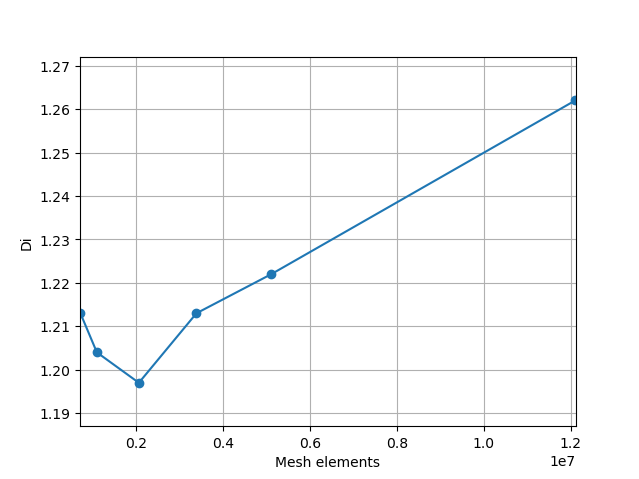
\includegraphics[width = 1\linewidth]{graphDi1}
        \caption{Зависимость диодности от разрешения сетки.}
        \label{fig:graphDi1}
    \end{figure}
    
    По графику (рис.~\ref{fig:graphDi1}) можно видеть, что с увеличением количества элементов сетки растет и диодность. Для того, чтобы сделать вывод о сеточной сходимости, нам надо добавить точек и выяснить, после какого разрешения диодность замедлит свой рост и последующее увеличении плотности расчетной сетки не будет давать значительного прироста точности. 
    \\
    %         \begin{table}[!htb]
        %            \begin{center}
            %                \caption{Результаты исследования сеточной сходимости с доп. точками.}
            %                 \begin{tabular}{rccc}
                %                     \hline
                %                     №      & Максимальный размер ячейки, мкм & Кол-во элементов сетки  & $Di$ \\
                %                     \hline
                %                     \hline
                %                     1	& 100		& 728 607		& 1,213		\\
                %                     2	& 80		& 1 106 796		& 1,204		\\
                %                     3  & 64		& 2 072 292		& 1,197		\\
                %                     4	& 51,2		& 3 395 988		& 1,213		\\
                %                     5	& 40,96		& 5 116 005		& 1,222		\\
                %                     6	& 40		& 5 602 384		& 1,287		\\
                %                     7	& 39,5		& 7 844 962		& 1,278		\\
                %                     8	& 39		& 9 039 949		& 1,288		\\
                %                     9	& 38		& 9 620 454		& 1,299		\\		
                %                     10	& 35		& 10 540 924	& 1,304		\\
                %                     11	& 32,768	& 12 107 251	& 1,262		\\
                %                     12	& 31,1296	& 12 896 528	& 1,311		\\
                %                     13	& 29,6		& 13 815 303	& 1,327		\\
                %                     14	& 28,6		& 14 401 893	& 1,310		\\
                %                     15	& 26		& 15 471 471	& 1,320		\\
                %                     16	& 25		& 16 085 501	& 1,330		\\
                %                     17	& 24	  	& 18 362 556	& 1,345		\\
                %                     18	& 23		& 22 476 068	& 1,327		\\
                %                     19	& 21		& 24 620 942	& 1,291		\\
                %                     20	& 19		& 28 765 237	& 1,3		\\
                %                     \hline
                %                     \label{fig:table2}
                %                 \end{tabular}
            %            \label{tab:tab2} 
            %            \end{center}
        %        \end{table}
    \\
    
    
    
    %         \begin{figure}[H]
        %             \centering
        %             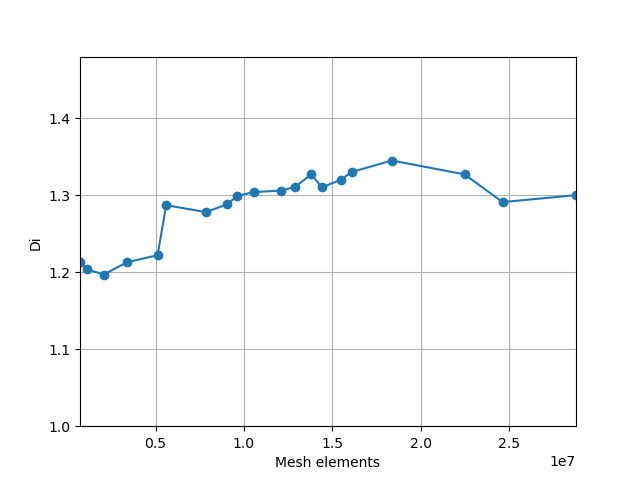
\includegraphics[width = 1\linewidth]{graphDi2}
        %             \caption{Зависимость диодности от разрешения сетки c доп. точками.}
        %             \label{fig:graphDi2}
        %         \end{figure}           
    
    \begin{figure}[H]
        \centering
        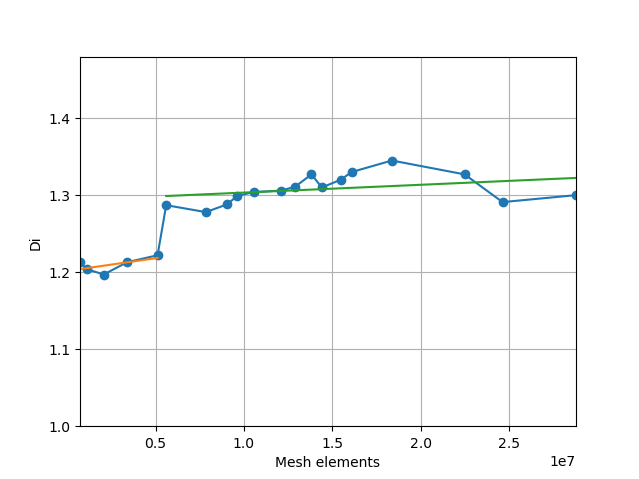
\includegraphics[width = 1\linewidth]{graphDiWithTrendLine}
        \caption{Линии тренда для зависимости диодности от количества элементов}
        \label{fig:graphDiWithTrendLine}
    \end{figure}         
    По представленным на графике (рис.~\ref{fig:graphDiWithTrendLine}) данным можно видеть, как с последующем увеличением разрешения сетки, диодность резко возрастает, однако, в последствии, рост диодности заметно замедляется. Исходя из этого, можно сделать вывод о сеточной сходимости. Достигая определенной плотности сетки, дальнейшее увеличение количества элементов не приведет к значительному улучшению решения, но потребует дополнительных вычислительных ресурсов. Добавленные линии тренда позволяют нам увидеть, что сетки до 5 млн элементов имеют рост диодности выше, чем сетки с более высокой плотностью, но среднее значение диодности у них меньше. Средний рост диодности для сеток с разрешением менее 5 миллионов элементов составляет 1,75 \textdiscount, в то время как для сеток с большим разрешением средний рост диодности составляет уже 0,99 \textdiscount. Если взять максимальное разрешение сетки за эталонное, то есть максимально приближенное к правильному решению, и посчитать во сколько процентов отличаются решения с меньшем разрешением, то результаты, полученные на сетках с разрешением менее 5 млн. элементов отличаются в более чем на 5 \textdiscount. Для дальнейшего параметрического исследования, нам следует выбрать сетку, плотность которой можно считать оптимальной. Для этого построим график зависимости диодности от максимального размера ячейки сетки.
            
    \begin{figure}[H]
        \centering
        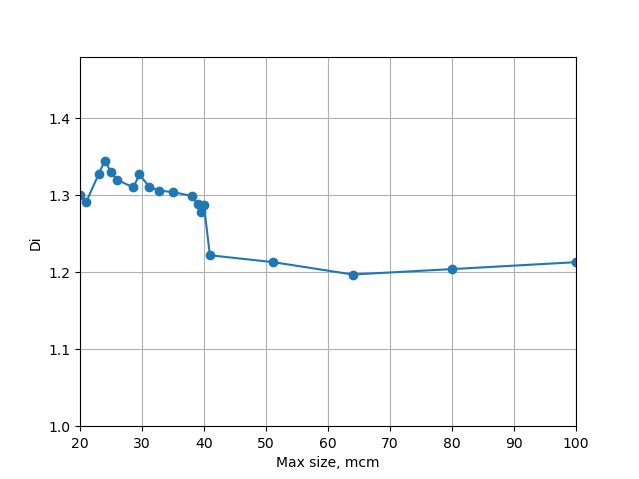
\includegraphics[width = 0.5\linewidth]{graphDiMaxSize}
        \caption{Зависимость диодности от максимального размера ячейки}
        \label{fig:graphDiMaxSize}
    \end{figure}
     
    Из графика (рис.~\ref{fig:graphDiMaxSize}) можно сделать вывод о том, что значительный прирост диодности происходит при максимальном характерном размере ячейки сетки равным 40 мкм. Этот размер мы и будем использовать при параметрическом исследовании. Что позволить нам получать более точные результаты оптимально задействовав вычислительные мощности. 
    
    
    Параметрическое исследование клапана Теслы. Был проведен ряд расчетов, используя оптимальную плотность сетки определенную в ходе исследования сеточной сходимости. В этих расчетах мы изменяли угол $ \alpha $ (рис.~\ref{fig:td}), определяя угол при котором диодность будет максимальной. Минимальное значение для угла $ \alpha $ равно 10\textdegree, а максимальное 70\textdegree. В ходе исследования, шаг для угла был взять равным 5\textdegree. В месте, с предполагаемым пиком диодности, 20\textdegree, шаг был равным 1,25\textdegree. 
    
    \begin{figure}[H]
        \centering
        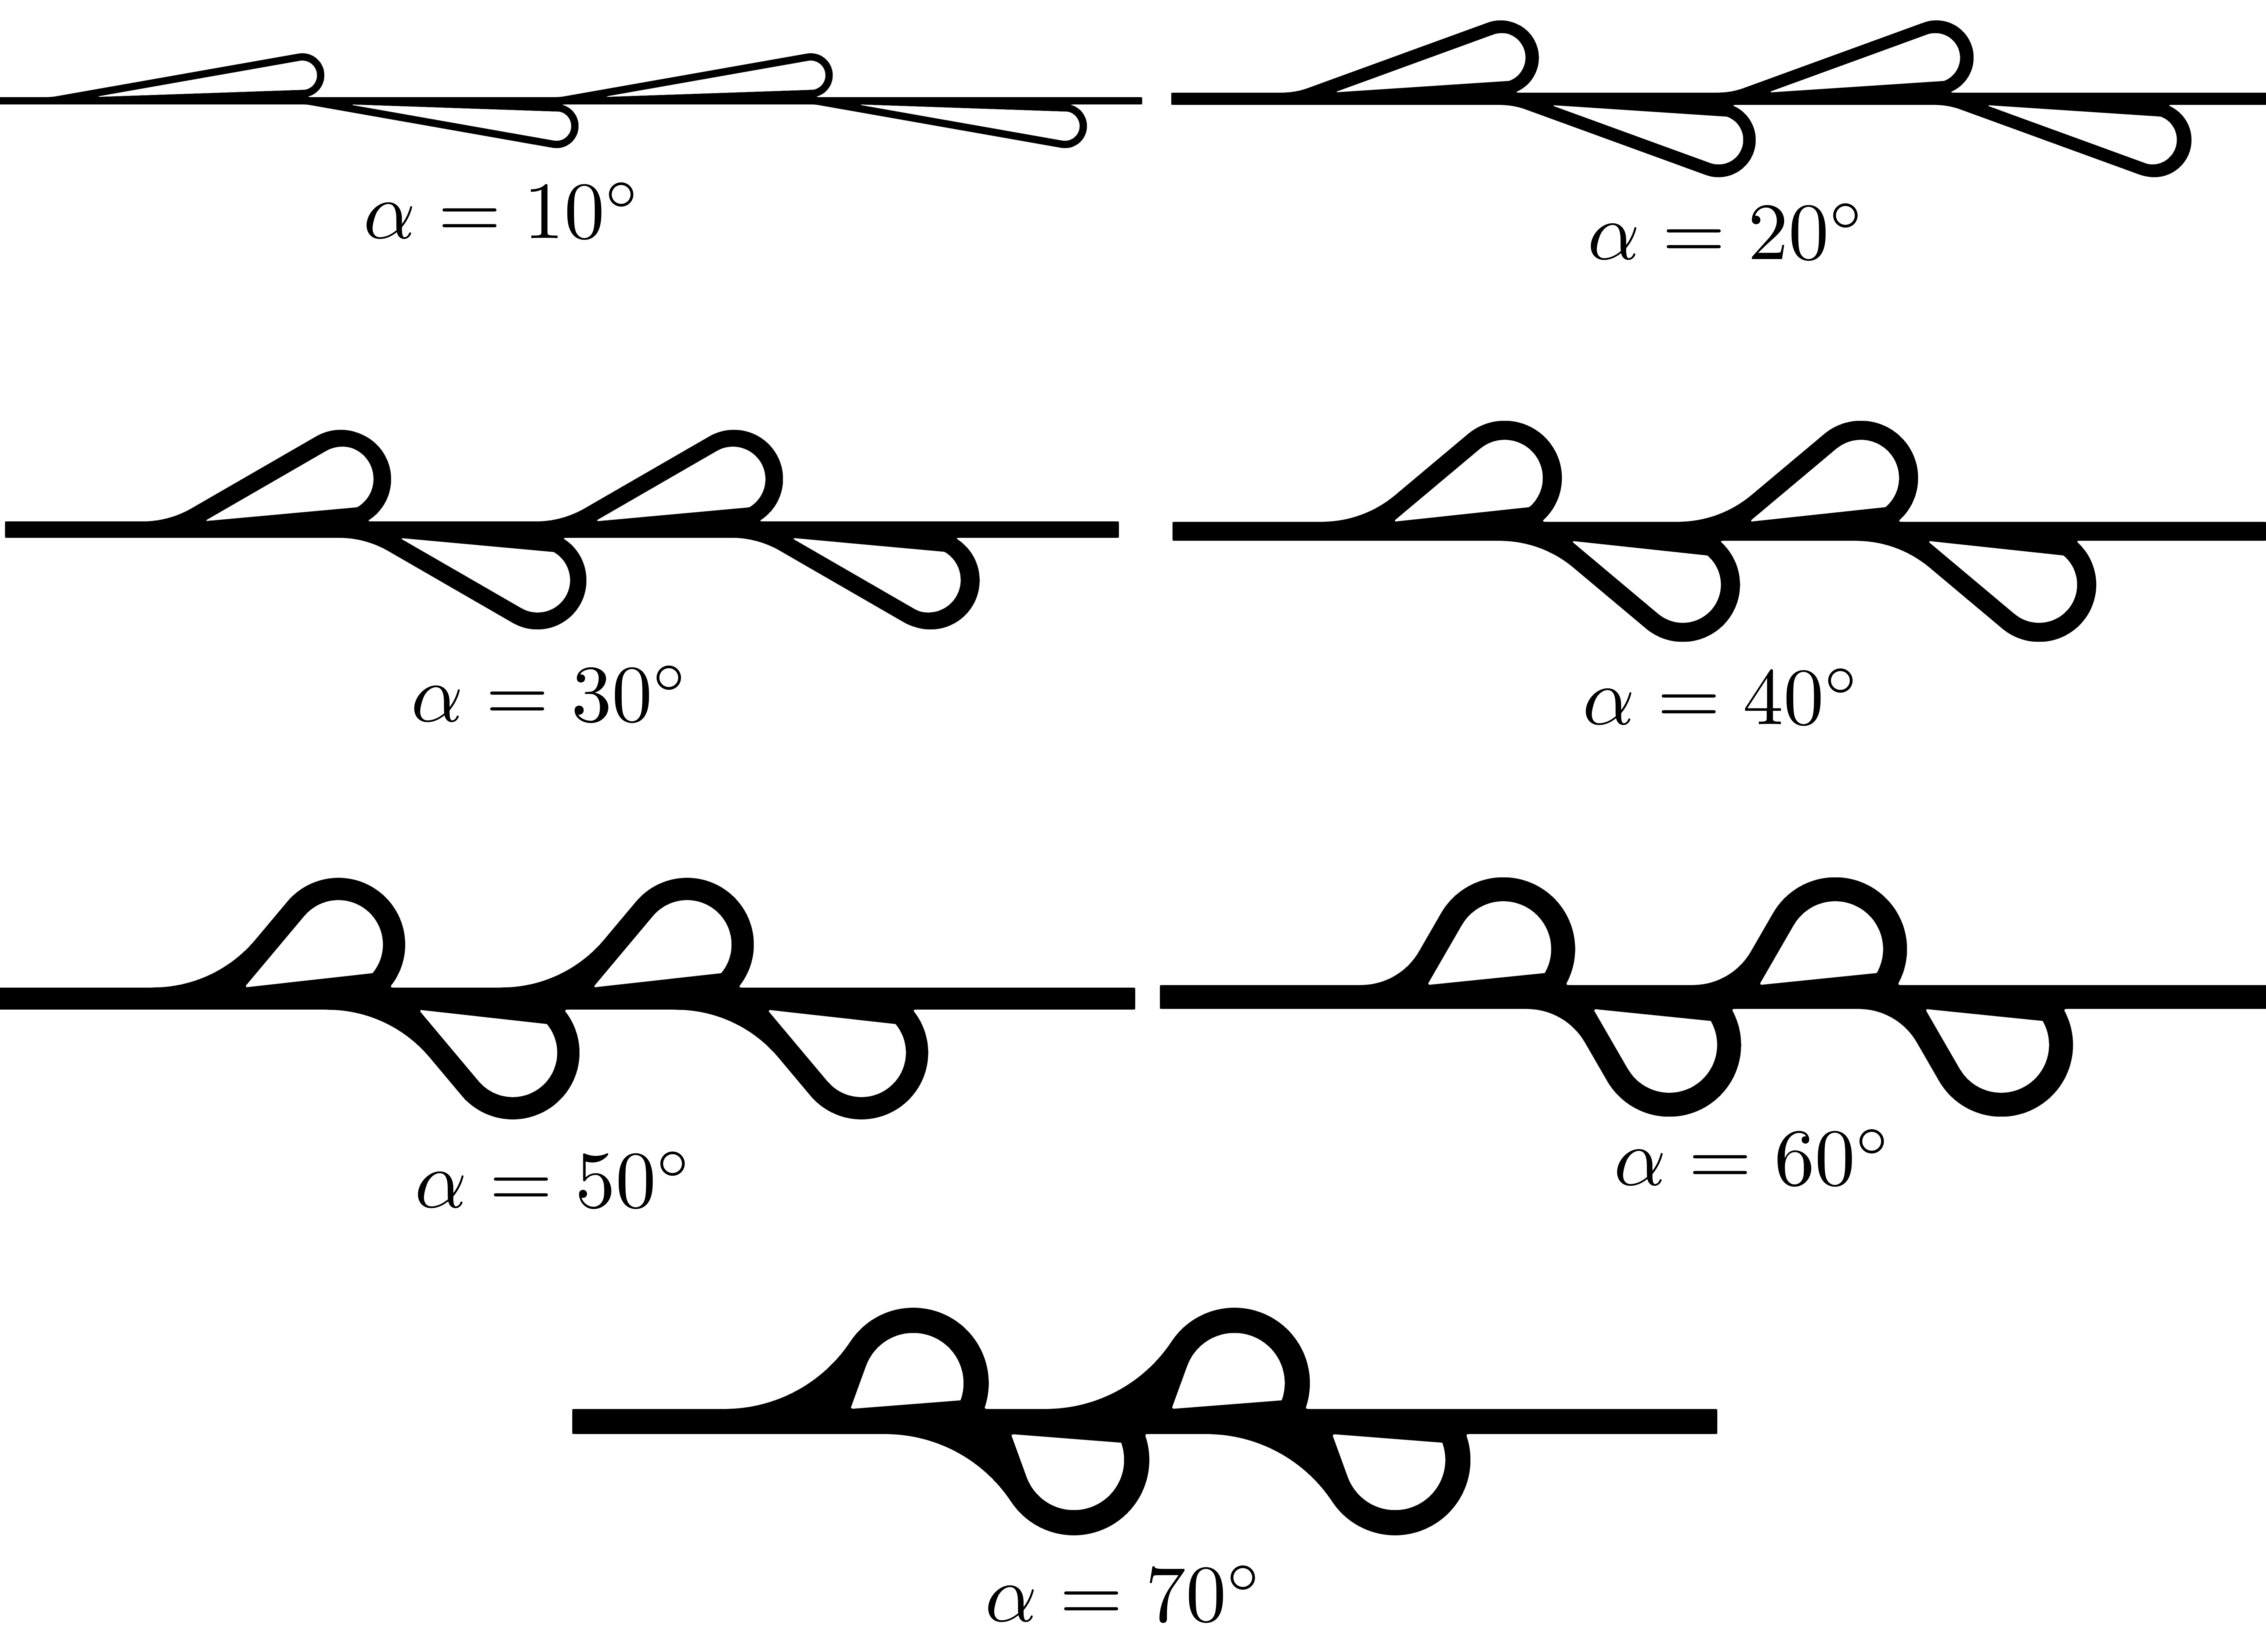
\includegraphics[width = 1\linewidth]{allAngle1}
        \caption{Построение геометрии при разном угле $\alpha$.}
        \label{fig:allAngle}
    \end{figure}  
          
    Видно, как изменение угла $\alpha$ влияет на общую длину основного и отводящего каналов (рис.~\ref{fig:allAngle}). Это значит, что при постоянной плотности сетки, количество её ячеек, как и требуемые вычислительные ресурсы, будет расти при уменьшении угла между основным и отводящим каналом. В результате параметрического исследования мы получаем следующий график (рис.~\ref{fig:alphaAngle}) зависимости диодности от угла $ \alpha $.
    
    %  ВСТАВИТЬ ФОТО ГЕОМЕТРИИ
    %  ОБЪЕДИНИТЬ ФОТО В ОДНО
    %   \\
    
    
    
    \begin{figure}[H]
        \centering
        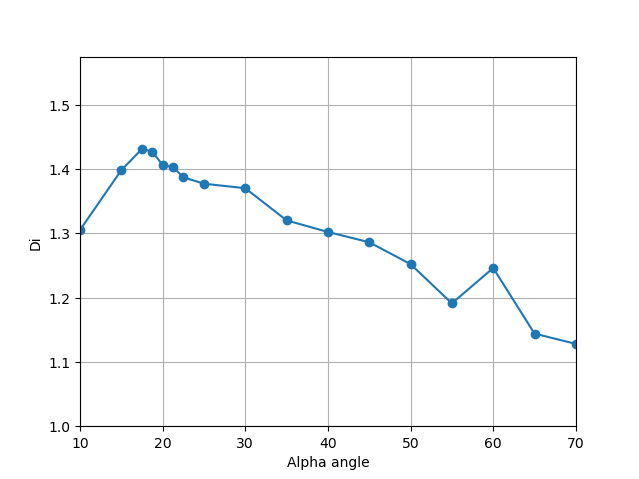
\includegraphics[width = 1\linewidth]{alphaAngle}
        \caption{Зависимость диодности от угла $\alpha$}
        \label{fig:alphaAngle}
    \end{figure}    
    В результате параметрического исследования было выяснено, что наша конфигурация клапана Теслы имеет максимальную диодность при угле $ \alpha $ равным 17,5 градуса. 
    
    \section{Выводы}
    
    Исследование сеточной сходимости показало, что при решении задач численными методами, важно соблюдать баланс между точностью решения и трат вычислительных ресурсов. Высокая точность требует больших затрат по времени и высокой производительности вычислительной техники. При проведении параметрического исследования нашей конфигурации клапана Теслы, был проведен ряд расчетов позволяющих резюмировать, что, при угле $\alpha$  = 17,5\textdegree, клапан Тесла нашей конфигурации имеет эффективность своей работы оцениваемую в $Di$ = 1,431.
    
    
    \vspace*{10mm plus 2mm minus 2mm}
    
    %=======================  Список литературы ==================================
    \LITERRUS
    
    %---------------------------------------------
    %Моя литература на русском (начало)
    %---------------------------------------------
    
    %1
    \rlitem{Algo500-1}{%1
        \textit{Antonov~A.S., Nikitenko~D.A., Voevodin~Vl.V.} 
        Algo500 --- a new approach to the joint analysis of
        algorithms and computers~//
        Lobachevskii J. Math. 2020. {\bf 41}, N~8. 1435--1443. 
        \doi{10.1134/S1995080220080041}.
    }
    
    
    
    
    
    %---------------------------------------------
    %Моя литература на русском (конец)
    %---------------------------------------------
    
    
    %=======================  Список литературы ======================
    \medskip
    
    \DateRU  
    
    \bigskip
    \bigskip
    
    \MakeAuthorsInfoRU
    
    
    %=========================== REFERENCES =========================
    \bigskip
    \bigskip
    
    
    \REFERENCES
    
    %---------------------------------------------
    %Моя литература на английском (начало)
    %---------------------------------------------
    
    %1
    \elitem{e:Algo500-1}{%1
        A.~S.~Antonov, D.~A.~Nikitenko, and Vl.~V.~Voevodin,
        ``Algo500 --- A New Approach to the Joint Analysis of Algorithms
        and Computers,''
        Lobachevskii J. Math. {\bf 41}~(8), 1435--1443 (2020).
        \doi{10.1134/S1995080220080041}.
    }
    
   
    
    %---------------------------------------------
    %Моя литература на английском (конец)
    %---------------------------------------------
    
    \medskip
    \DateEN
    
    \bigskip
    \bigskip
    \bigskip
    
    \MakeAuthorsInfoEN
    
    %============================ КОНЕЦ СТАТЬИ ==================================
    \end{document}